
% Due thursday

\documentclass{article}

\usepackage[utf8]{inputenc}

\usepackage{amsmath, bm}
\usepackage{graphicx}
\usepackage{amssymb}
\usepackage{float}
\usepackage{caption}
\usepackage{subcaption}
\usepackage{hyperref}
\usepackage{tikz}
\usepackage{layout}
\usepackage[export]{adjustbox}

\usepackage[margin=1in]{geometry}
\usepackage{listings}
\usepackage{xcolor}
\usepackage{color, colortbl}
\usepackage{textgreek}
\usepackage{mathrsfs}
\usepackage{savetrees}


\setlength{\parskip}{\baselineskip}%
\setlength{\parindent}{0pt}%
\linespread{0.9}


\definecolor{codegreen}{rgb}{0,0.6,0}
\definecolor{codegray}{rgb}{0.5,0.5,0.5}
\definecolor{codepurple}{rgb}{0.58,0,0.82}
\definecolor{backcolour}{rgb}{0.95,0.95,0.92}

\lstdefinestyle{mystyle}{
    backgroundcolor=\color{backcolour},   
    commentstyle=\color{codegreen},
    keywordstyle=\color{magenta},
    numberstyle=\tiny\color{codegray},
    stringstyle=\color{codepurple},
    basicstyle=\ttfamily\footnotesize,
    breakatwhitespace=false,         
    breaklines=true,                 
    captionpos=b,                    
    keepspaces=true,                 
    numbers=left,                    
    numbersep=5pt,                  
    showspaces=false,                
    showstringspaces=false,
    showtabs=false,                  
    tabsize=2
}

\lstset{style=mystyle}



\begin{document}

\title{SA1: Wing Analysis Final Report}
\author{lwp26}
\date{June 2024}
\maketitle 

\section{Introduction}
\subsection{Purpose}

\subsection{Objectives}

\section{Development of Software Tool}

\subsection{Panel Method}

Many of the panel method functions could be vectorized to improve performance.
\subsubsection{Single Panel}

\begin{figure}[H]
    \centering
    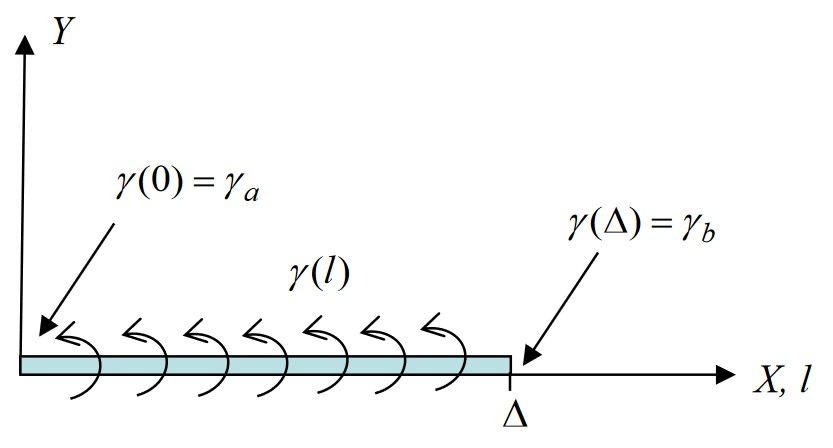
\includegraphics[width=0.3\textwidth]{figures/single_panel.jpg}
    \caption{Single Panel}
    \label{fig:single_panel}
\end{figure}
The streamfunction due to a linearly distributed vortex panel is given by
\begin{equation}
    \psi(X,Y) = \gamma_a f_a + \gamma_b f_b
\end{equation}
where $f_a$ and $f_b$ are influence coefficients of the panel at points $a$ and $b$ respectively.
The influence functions can be found by integrating the Biot-Savart law over the panel.

A function is written to calculate the influence coefficients for a vector of panel points.


\subsection{Boundary Layer Solver}

\begin{figure}[H]
    \centering
    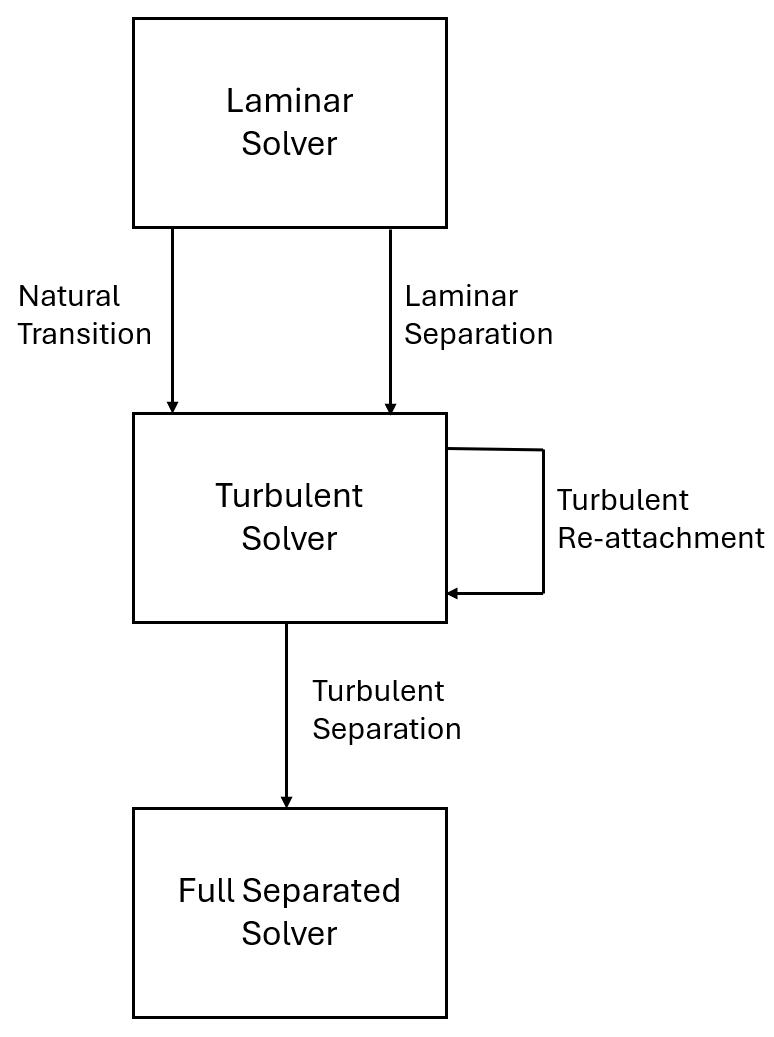
\includegraphics[width=0.2\textwidth]{figures/bl_solver_flowchart.png}
    \caption{Boundary Layer Profile}
    \label{fig:BL}
\end{figure}

\subsubsection{Laminar Regime}

Test for transition to turbulence
\begin{equation}
    \ln(Re_\theta) = 18.4 H_E - 21.74 \quad \text{ where } \quad Re_\theta = Re_L\left( \frac{u_e}{U} \right) \left( \frac{\theta}{L} \right)
\end{equation}

\begin{equation}
    m = - \frac{\theta^2}{\mu}\frac{du_e}{dx} = -Re_L \left( \frac{\theta}{L} \right)^2 \frac{d(u_e / U)}{d(x/L)}
\end{equation}

If $m > 0.09$, then the laminar boundary layer seperates and is treated as turbulent.

\subsubsection{Turbulent Regime}

\begin{equation}
    \dot{\mathbf{y}} = \begin{bmatrix}
        \frac{d \theta}{d x} \\[5pt]
        \frac{d \delta_E}{d x}
    \end{bmatrix} = f(x,\mathbf{y}) = \begin{bmatrix}
        \frac{c_f}{2} - \frac{H+2}{u_e}\frac{d u_e}{d x} \theta \\[5pt]
        c_\text{diss} - \frac{3}{u_e} \frac{d \delta_E}{d x} \delta_E
    \end{bmatrix}
\end{equation}

\begin{align}
    H &= \begin{cases}
        \frac{11 H_E + 15}{48H_E - 59} & \text{if } H_E  \ge 1.46 \\
        2.803 & \text{if } H_E < 1.46
    \end{cases} \\
    c_f &= 0.091416\left[(H-1)Re_\theta \right]^{-0.232}e^{-1.26H} \\
    c_\text{diss} &= 0.010024\left[(H-1)Re_\theta \right]^{1/6}
\end{align}

\section{Software Performance}

\begin{figure}[H]
    \centering
    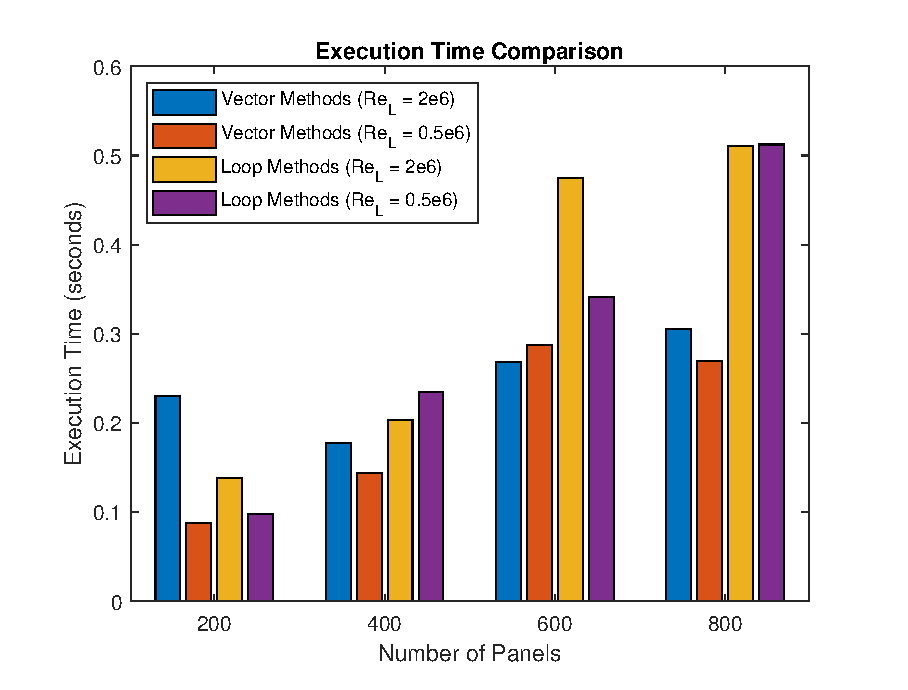
\includegraphics[width=0.6\textwidth]{figures/RePanelVec_times.eps}
    \caption{Computation time for NACA 0012 airfoil for varying number of panels, low and high Reynolds numbers, vectorized and loop algorithms at $\alpha = 5^\circ$}
    \label{fig:airfoil}
\end{figure}


\begin{figure}[H]
    \centering
    \captionsetup{justification=centering}
    \begin{subfigure}{0.45\textwidth}
        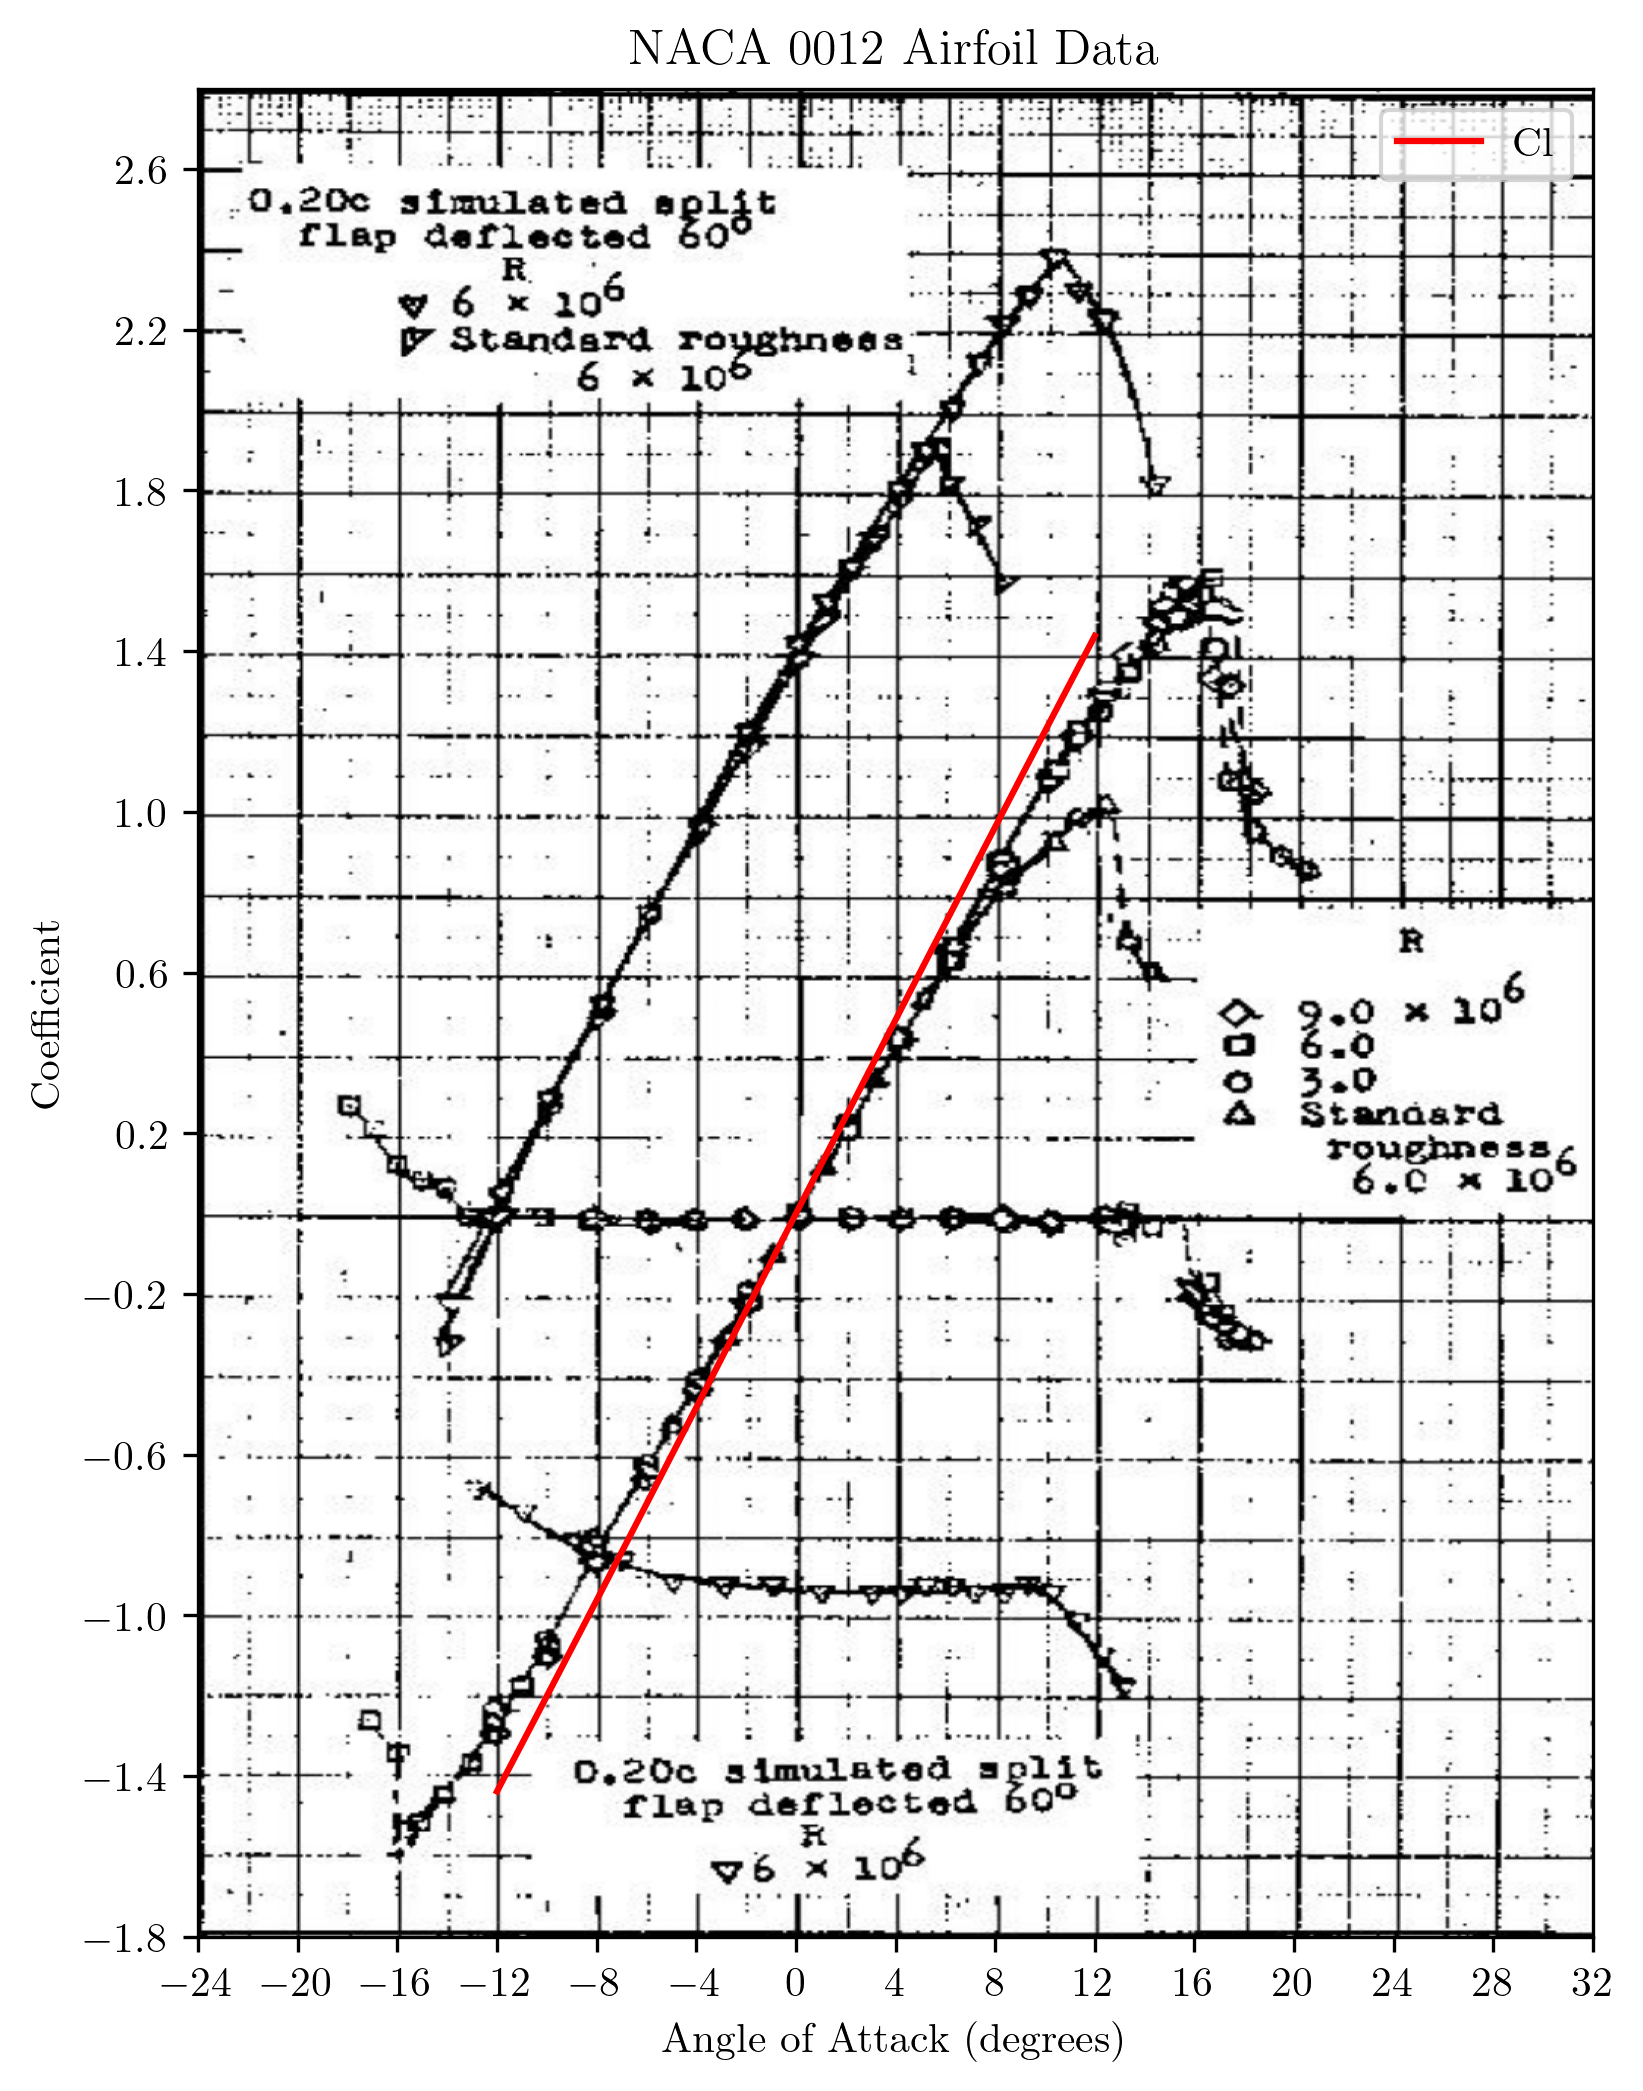
\includegraphics[width=0.99\textwidth]{figures/NACA0012_lift_validation.png}
        \caption{Lift coefficient against angle of attack}
        \label{fig:0012_lift_validation}
    \end{subfigure}
    \begin{subfigure}{0.45\textwidth}
        \centering
        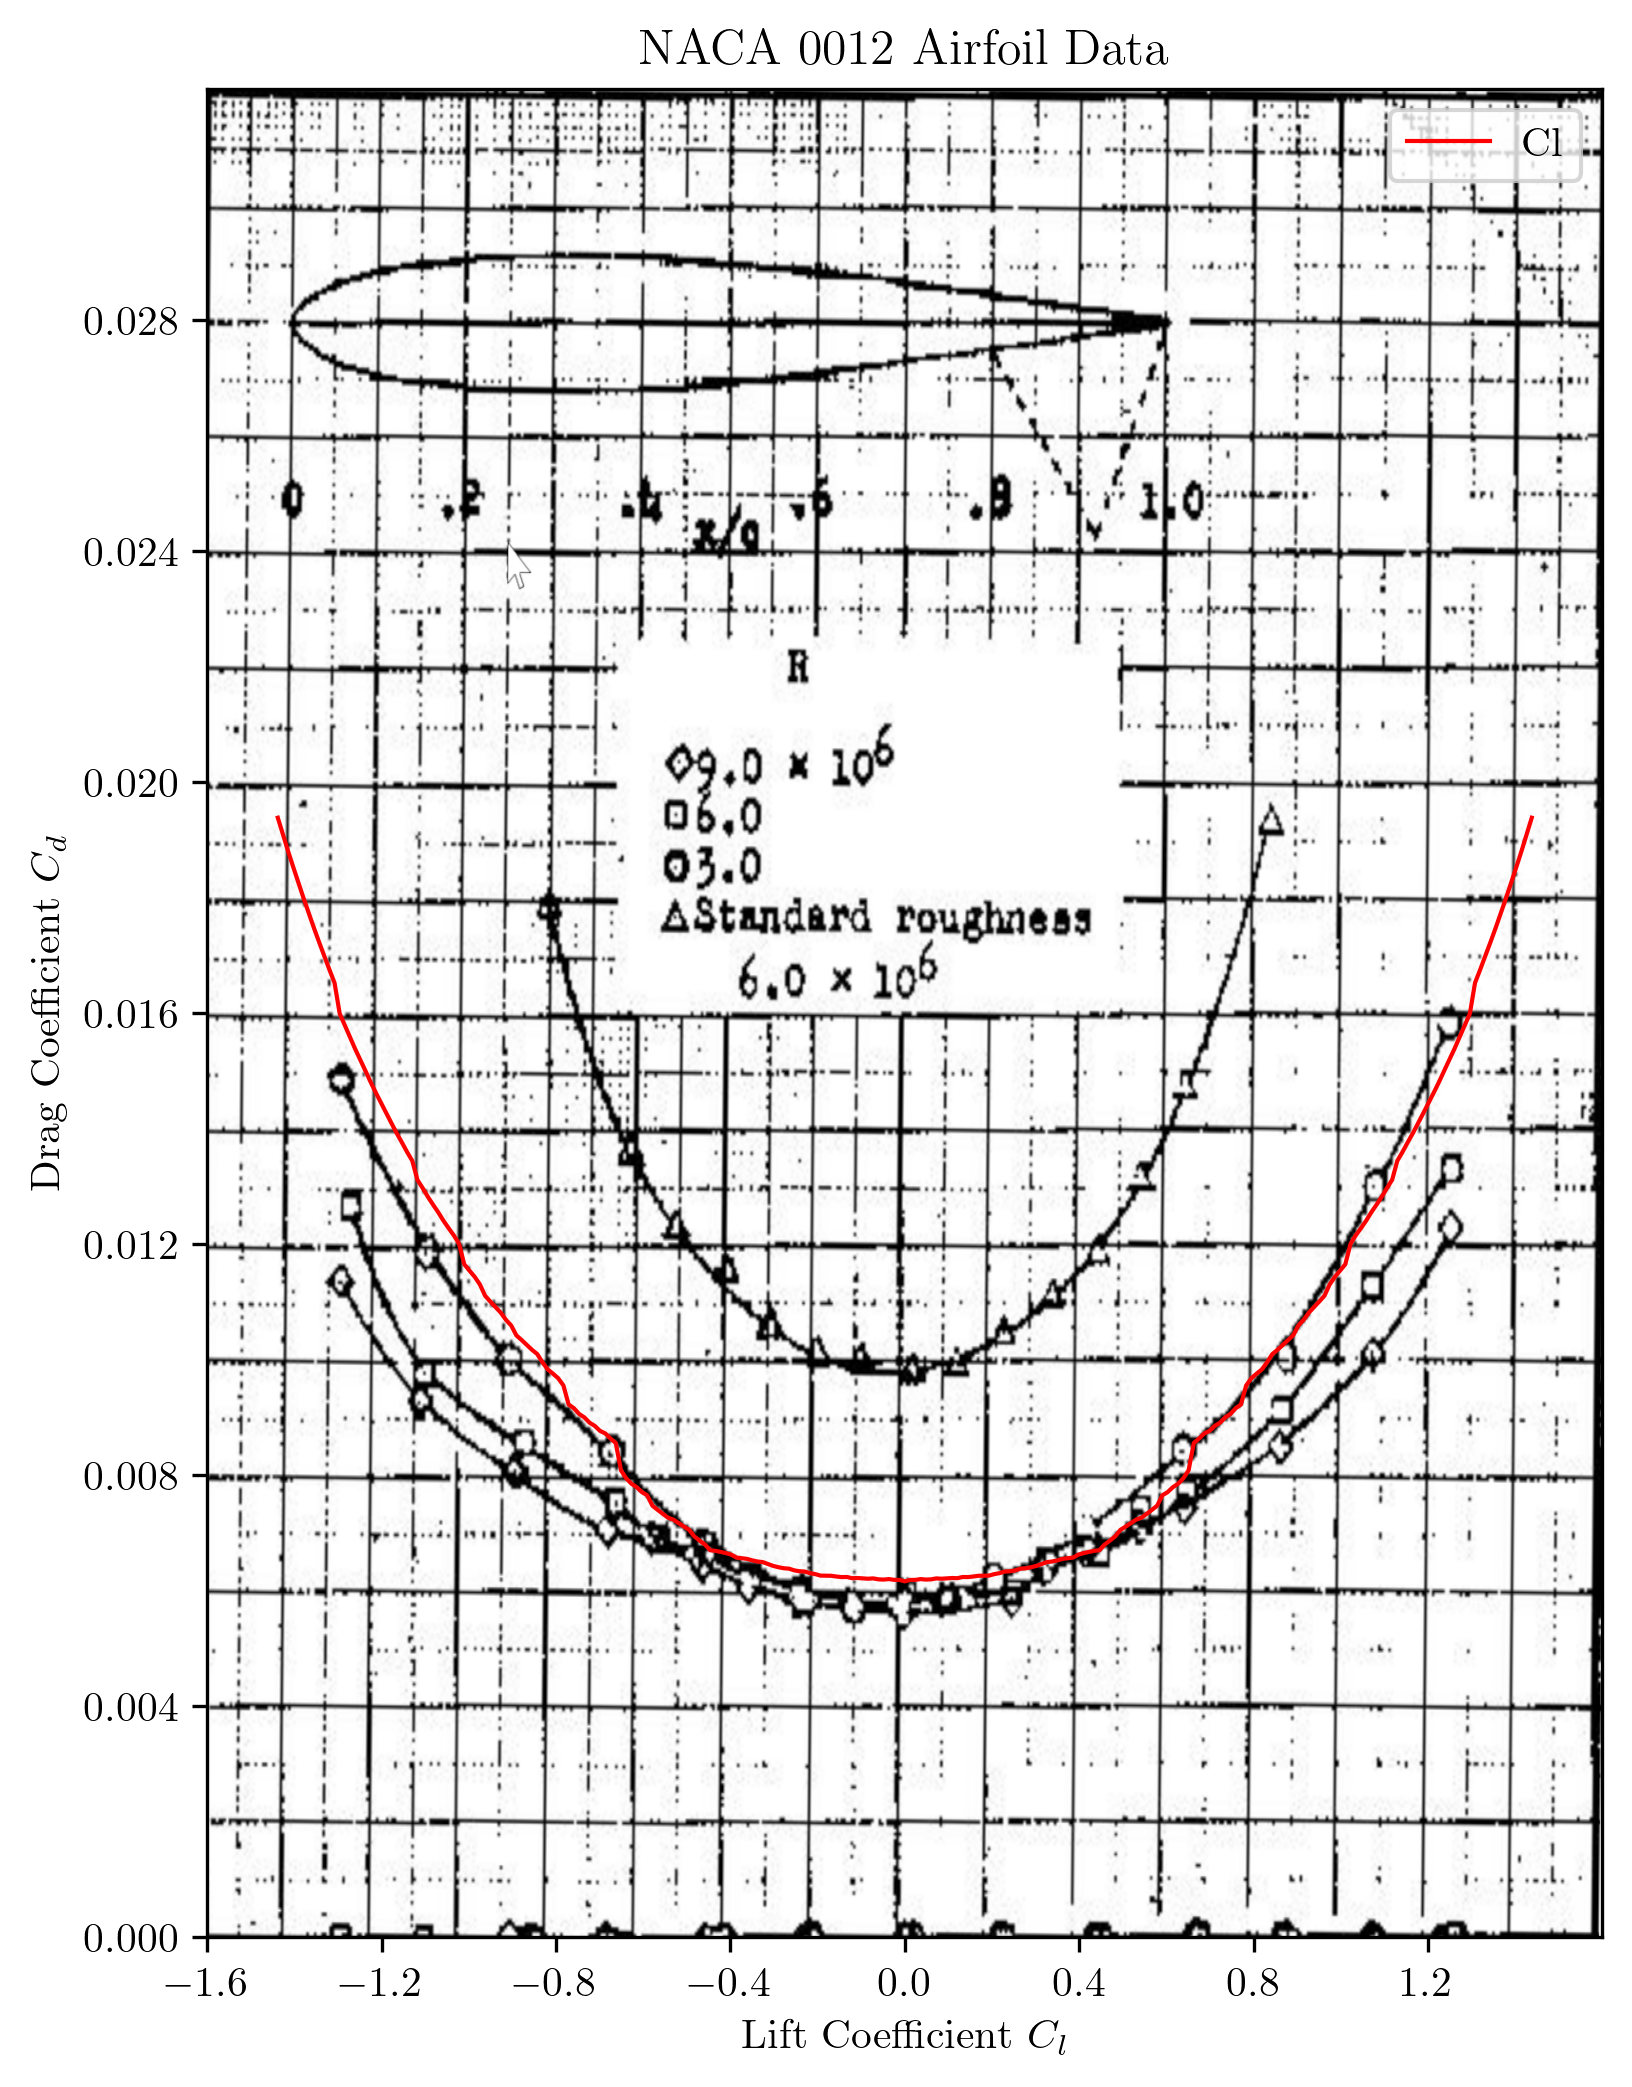
\includegraphics[width=0.99\textwidth]{figures/NACA0012_drag_validation.png}
        \caption{Drag coefficient against lift coefficient}
        \label{fig:0012_drag_validation}
    \end{subfigure}
    \caption{Experimetnal and calculated performance at $Re = 3\times10^6$ for the NACA0012 aerofoil}
\end{figure}

\begin{figure}[H]
    \centering
    \captionsetup{justification=centering}
    \begin{subfigure}{0.45\textwidth}
        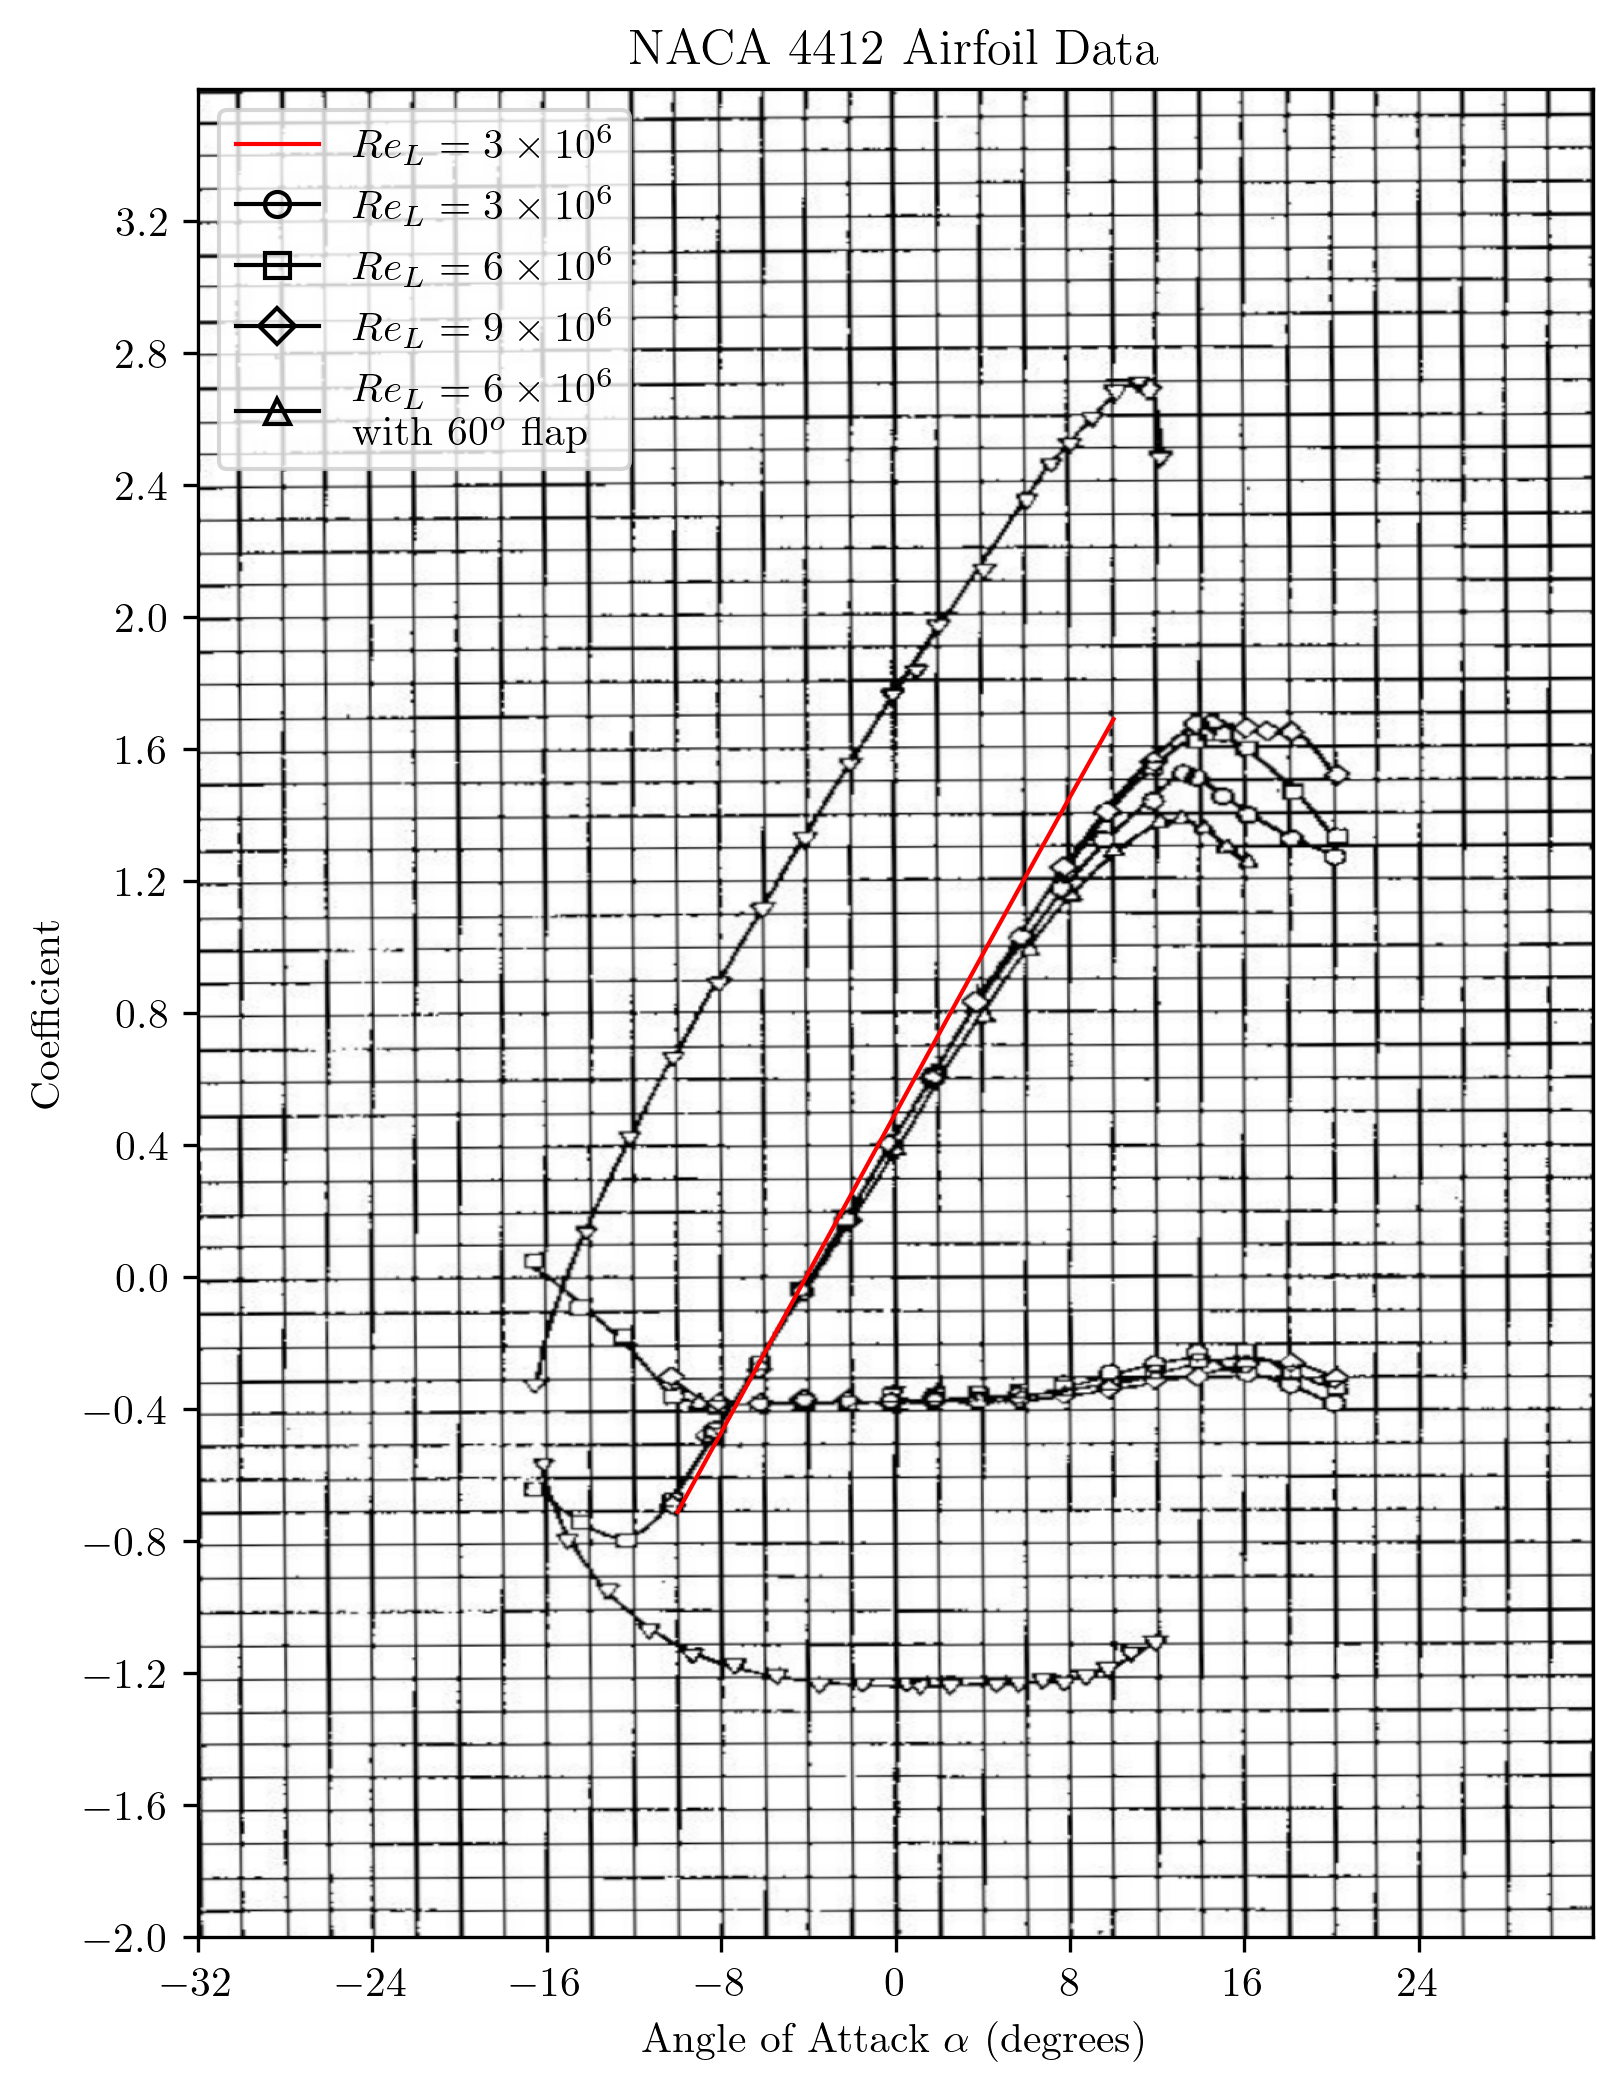
\includegraphics[width=0.9\textwidth]{figures/NACA4412_lift_validation.png}
        \caption{Lift coefficient against angle of attack}
        \label{fig:4412_lift_validation}
    \end{subfigure}
    \begin{subfigure}{0.45\textwidth}
        \centering
        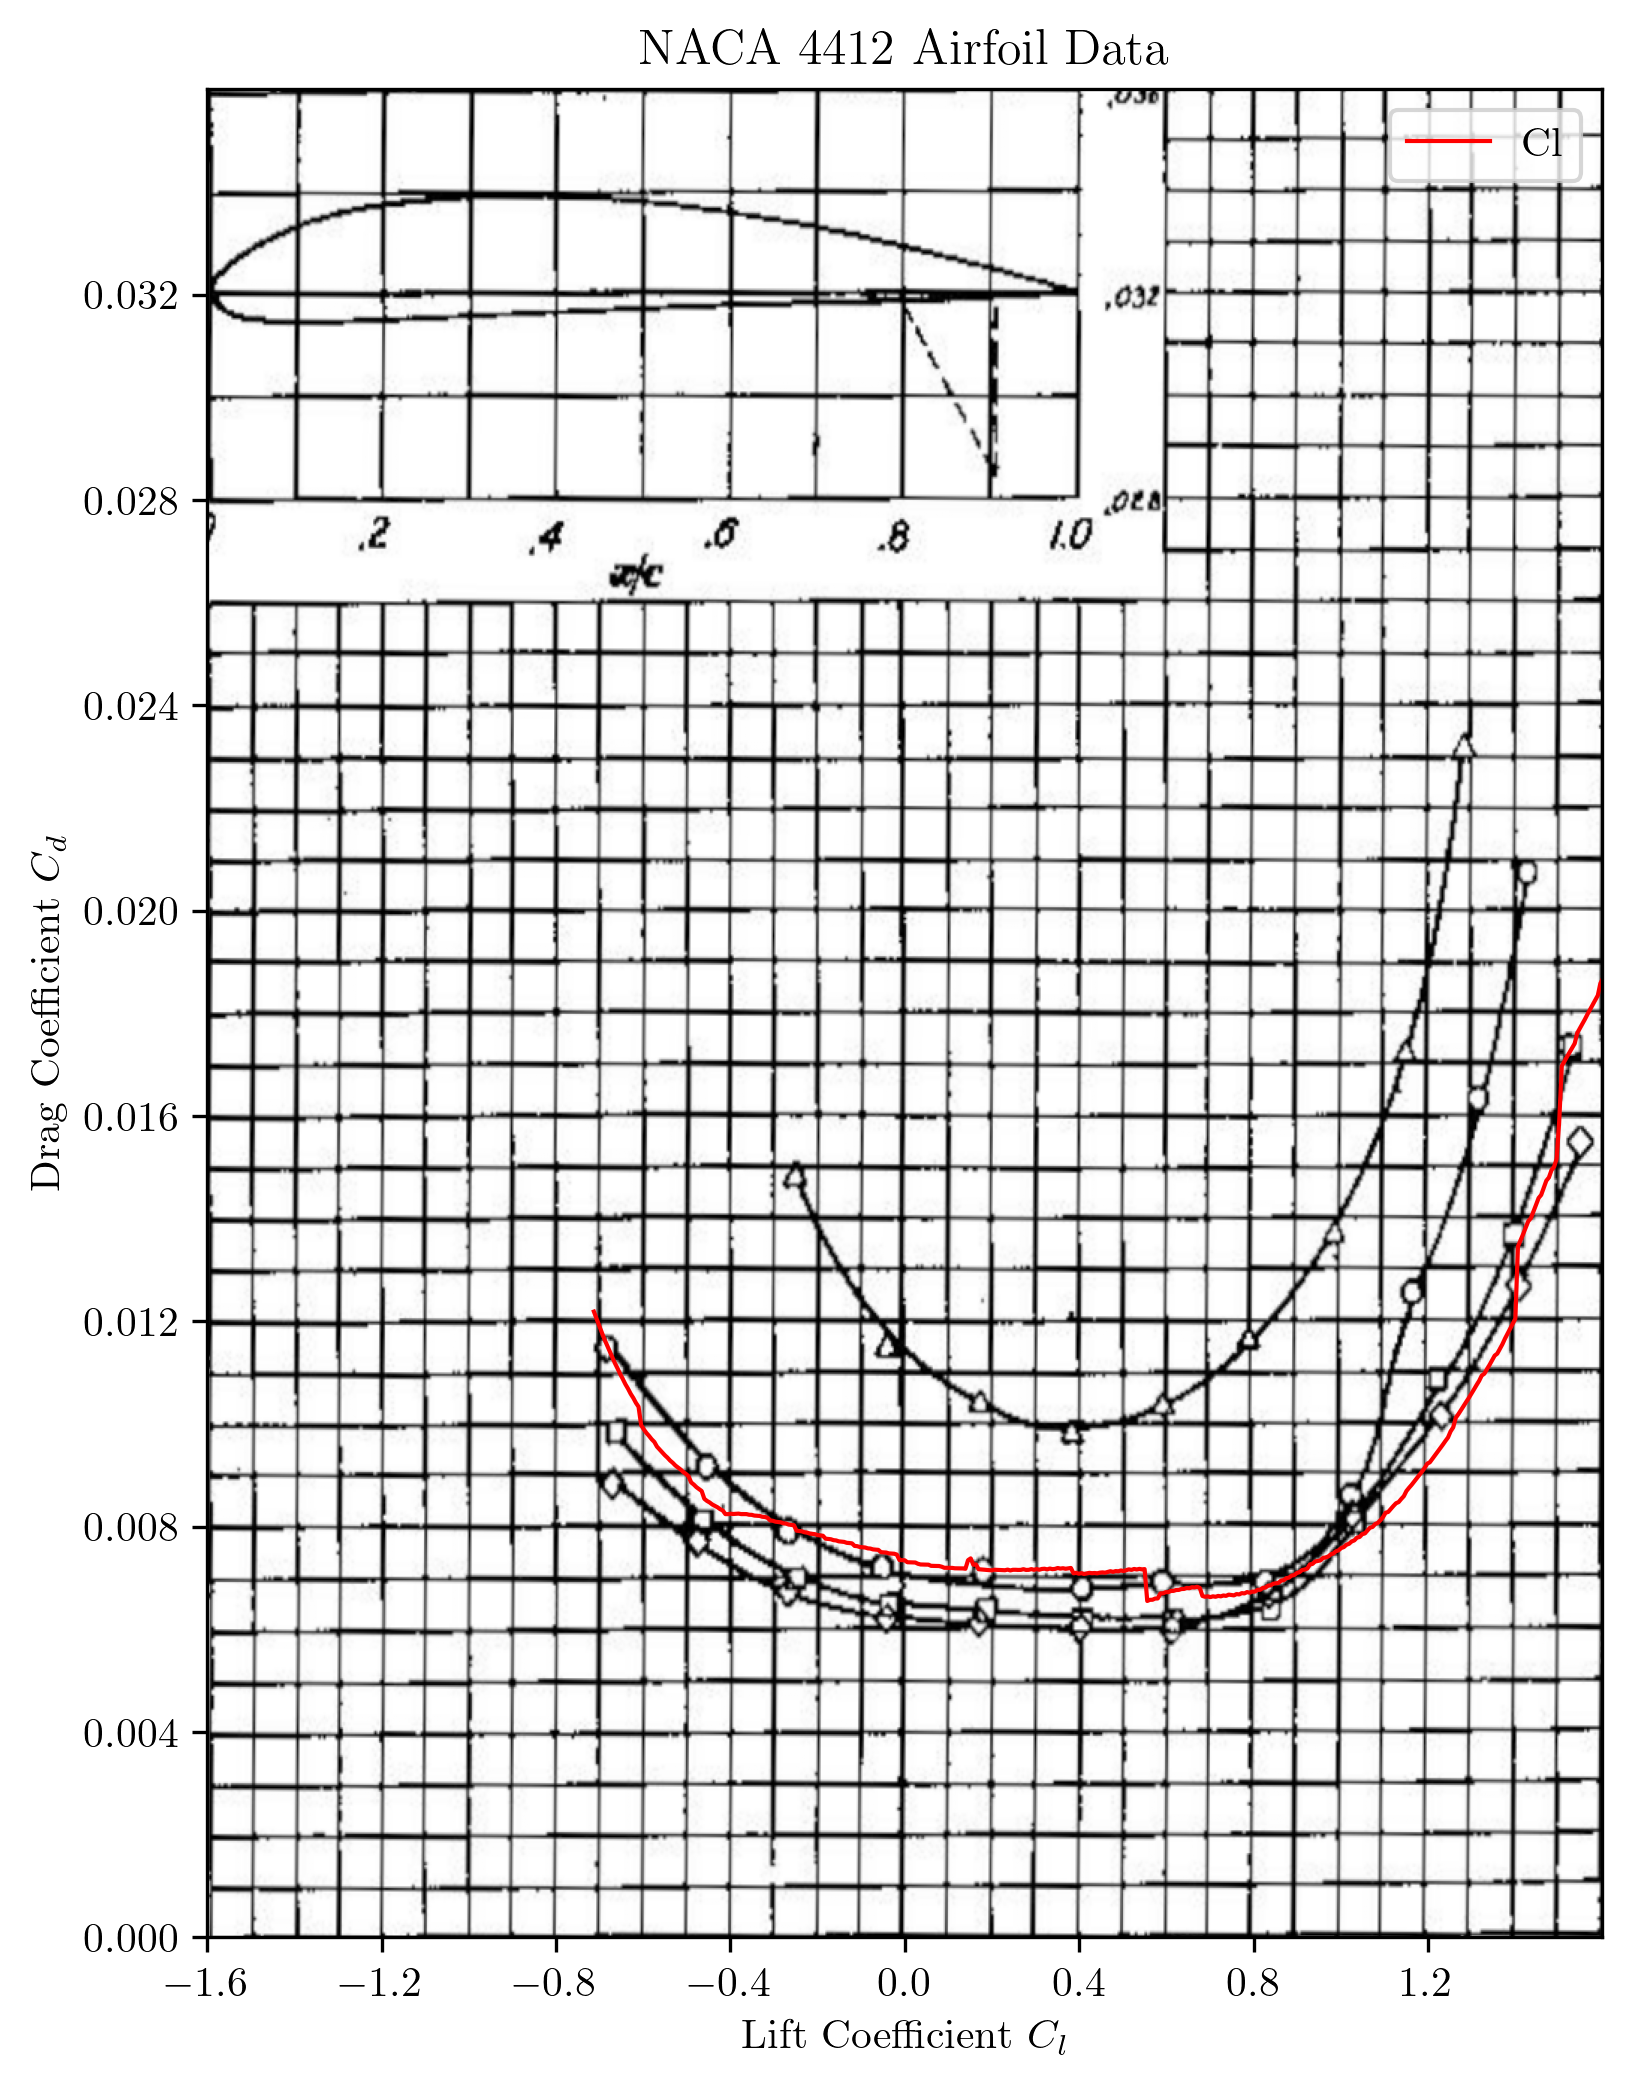
\includegraphics[width=0.9\textwidth]{figures/NACA4412_drag_validation.png}
        \caption{Drag coefficient against lift coefficient}
        \label{fig:4412_drag_validation}
    \end{subfigure}
    \caption{Experimetnal and calculated performance at $Re = 3\times10^6$ for the NACA4412 aerofoil}
\end{figure}

\section{Topology Optimization}

\subsection{Changing Topology}

A spline fit tool is used to paramaterize complex curves with a small number of control points.
The calculated lift and drag coefficients are very sensitive to control point position.

\subsection{High Reynolds Number}

\begin{figure}[H]
    \centering
    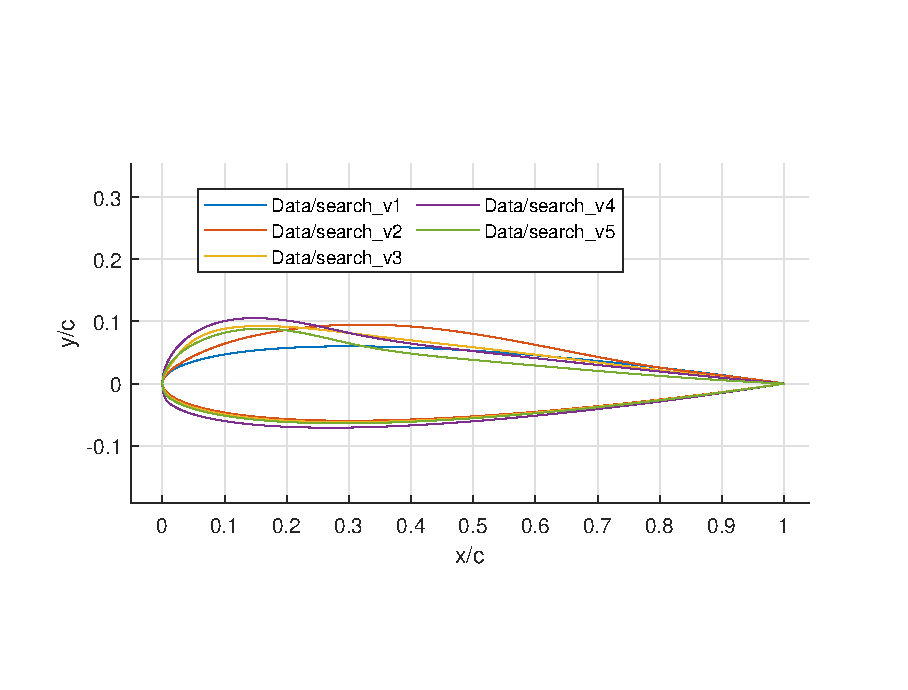
\includegraphics[width=0.8\textwidth]{figures/hiRe_geometry_5.eps}
    \caption{Airfoil Geometry of first 5 design iterations}
    \label{fig:v5_geometry}
\end{figure}

\begin{figure}[H]
    \centering
    \begin{subfigure}{0.45\textwidth}
        \centering
        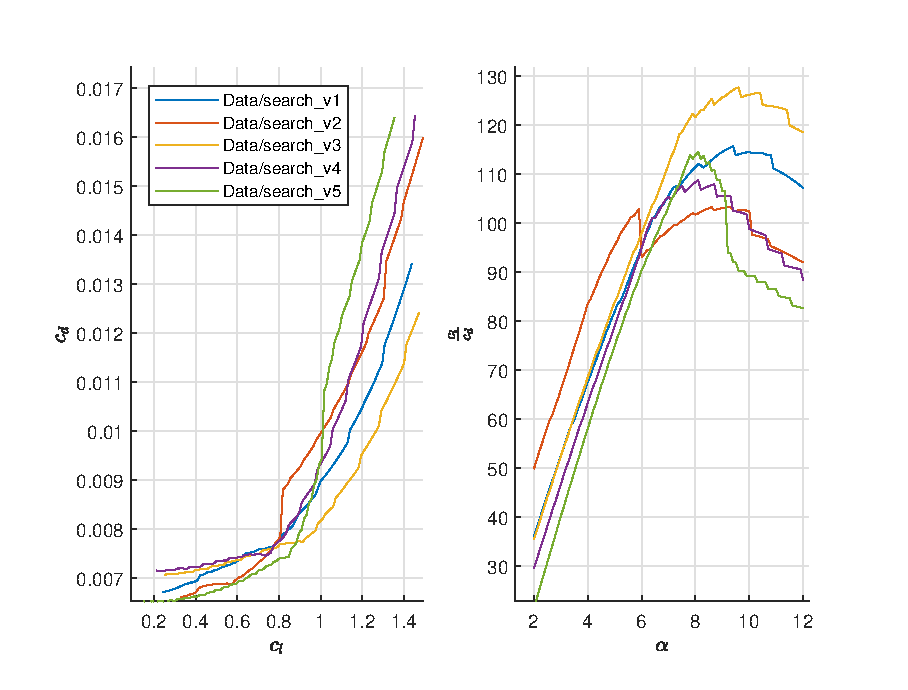
\includegraphics[width=1.2\textwidth, center]{figures/hiRe_lod_5.eps}
        \caption{Airfoil}
        \label{fig:v5_lod}
    \end{subfigure}
    \begin{subfigure}{0.54\textwidth}
        \centering
        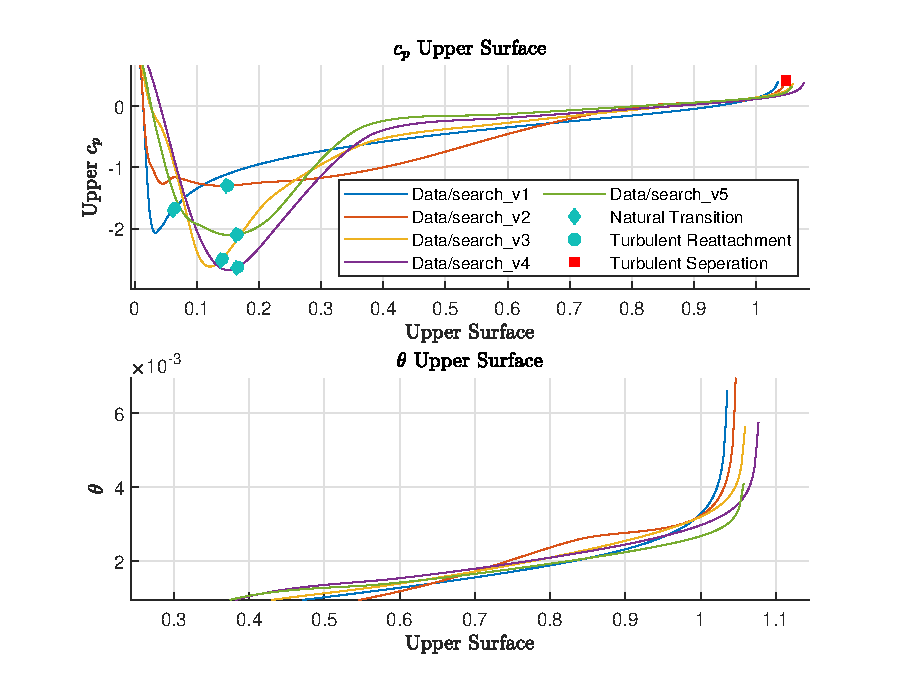
\includegraphics[width=0.99\textwidth]{figures/hiRe_upperprofile_5_a5.eps}
        \caption{Pressure coefficient and momentum thickness profiles for $\alpha = 5^\circ$}
        \label{fig:v5_profile}
    \end{subfigure}
    \caption{Performance of initial 5 design iterations and their upper surface boundary layer profiles}
\end{figure}

\begin{figure}[H]
    \centering
    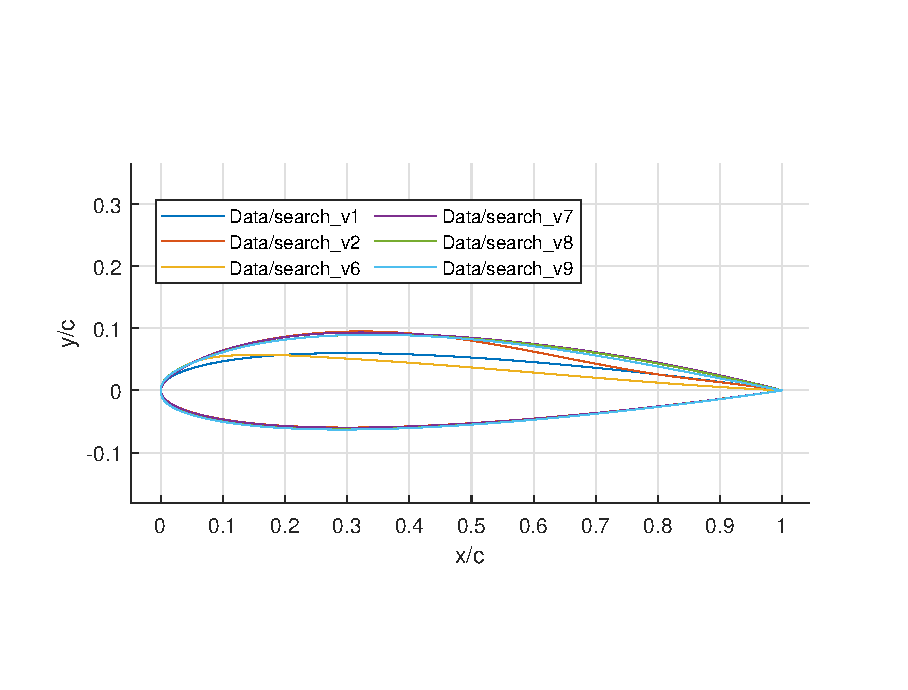
\includegraphics[width=0.8\textwidth]{figures/hiRe_geometry_9.eps}
    \caption{Airfoil Geometry}
    \label{fig:v9_geometry}
\end{figure}

\begin{figure}[H]
    \centering
    \begin{subfigure}{0.45\textwidth}
        \centering
        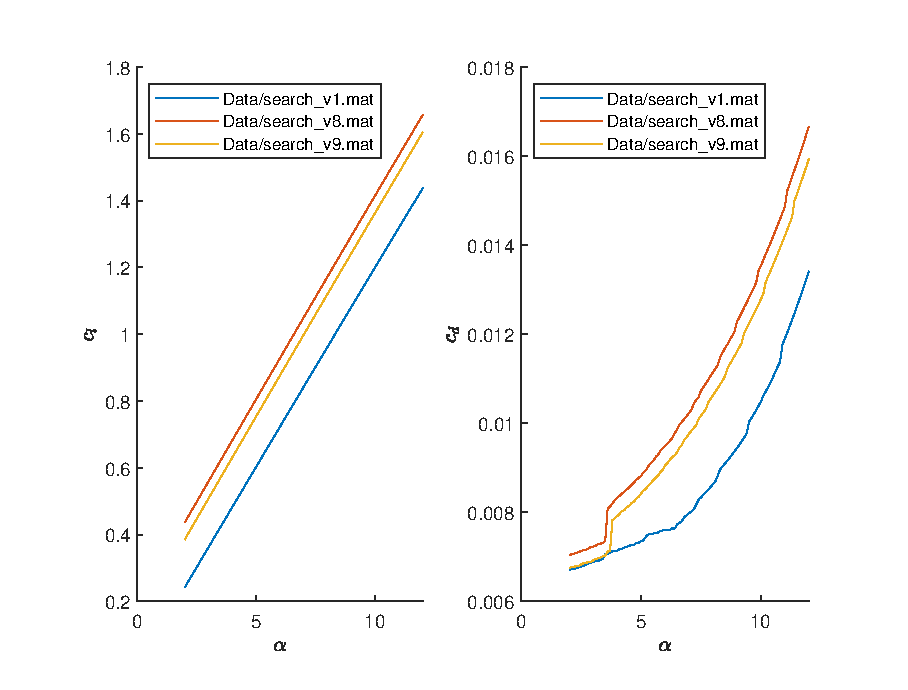
\includegraphics[width=1.2\textwidth, center]{figures/hiRe_lad_9.eps}
        \caption{Airfoil}
        \label{fig:v9_lod}
    \end{subfigure}
    \begin{subfigure}{0.54\textwidth}
        \centering
        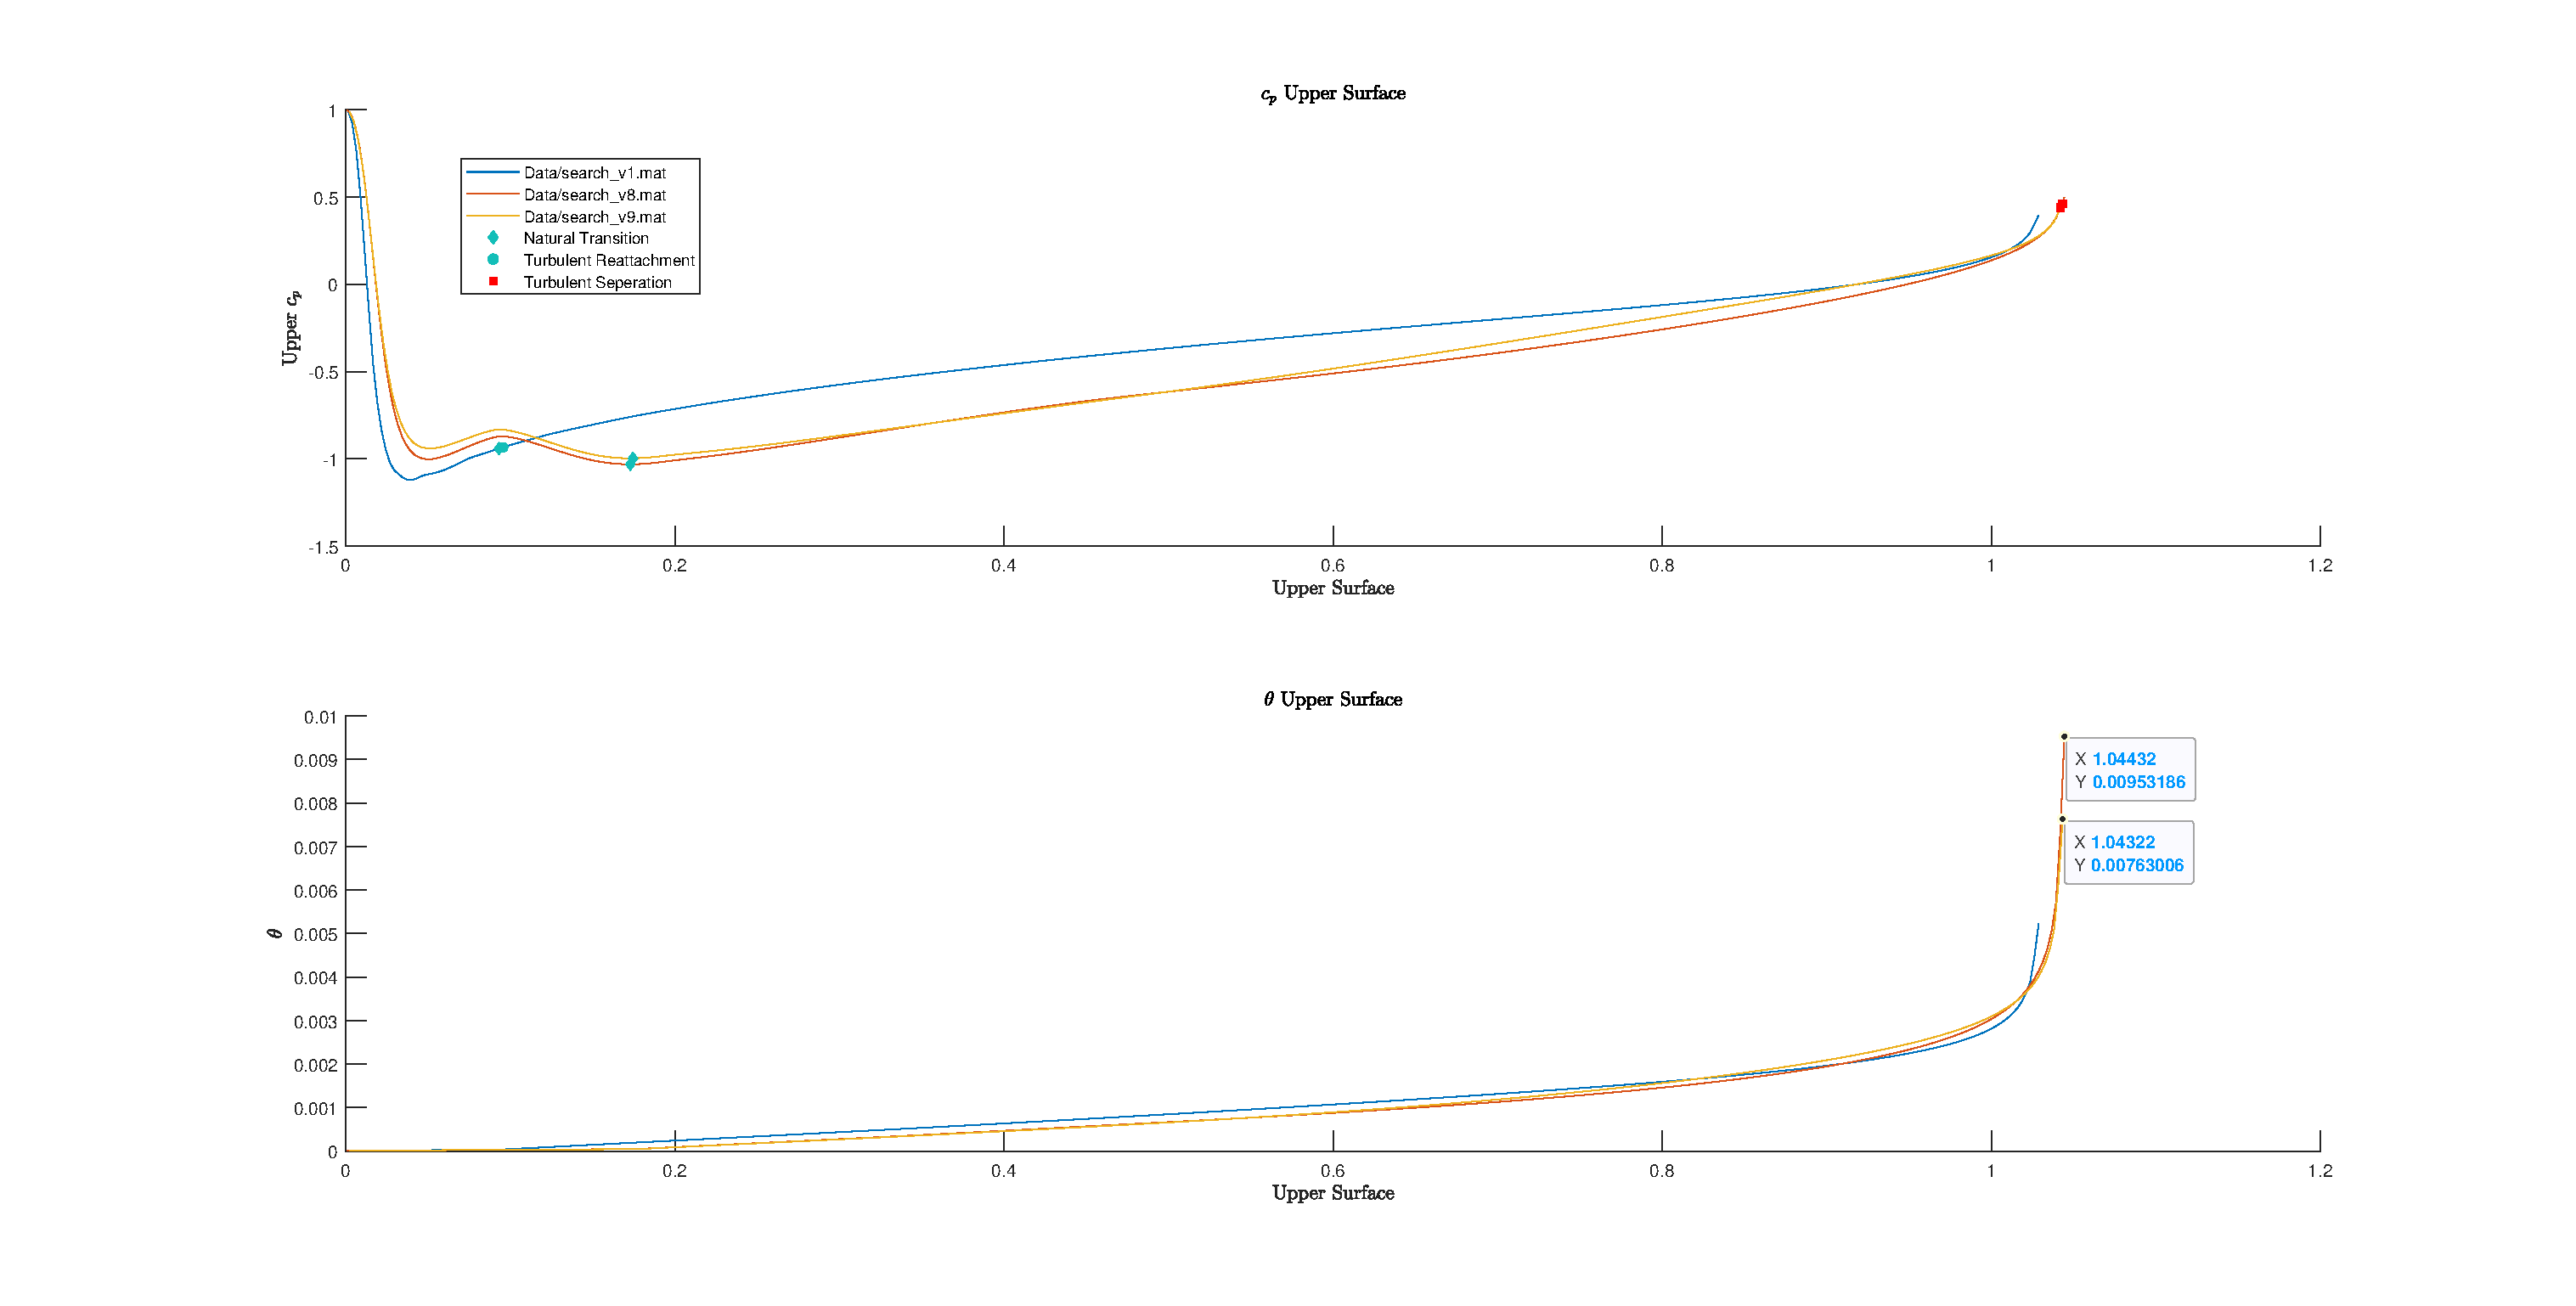
\includegraphics[width=0.99\textwidth]{figures/hiRe_upperprofile_9_a3.eps}
        \caption{Pressure coefficient and momentum thickness profiles for $\alpha = 3^\circ$}
        \label{fig:v9_profile}
    \end{subfigure}
    \caption{Performance of design iterations 6-9 and their upper surface boundary layer profiles}
\end{figure}

\begin{figure}[H]
    \begin{subfigure}{0.54\textwidth}
        \centering
        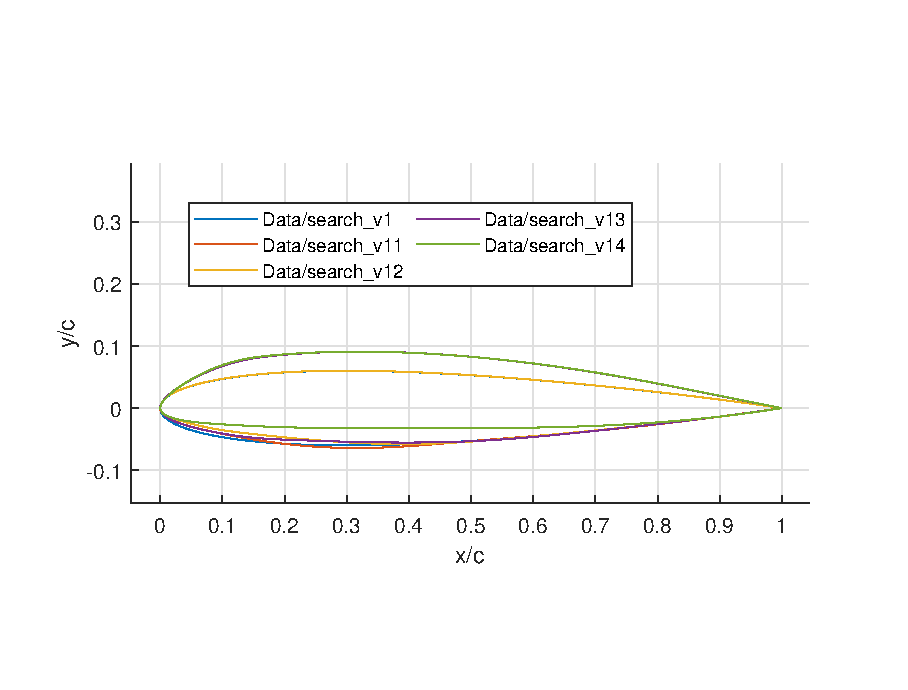
\includegraphics[width=1.2\textwidth, center]{figures/hiRe_geometry_14.eps}
        \caption{Airfoil Geometry}
        \label{fig:v14_geometry}
    \end{subfigure}
    \begin{subfigure}{0.45\textwidth}
        \centering
        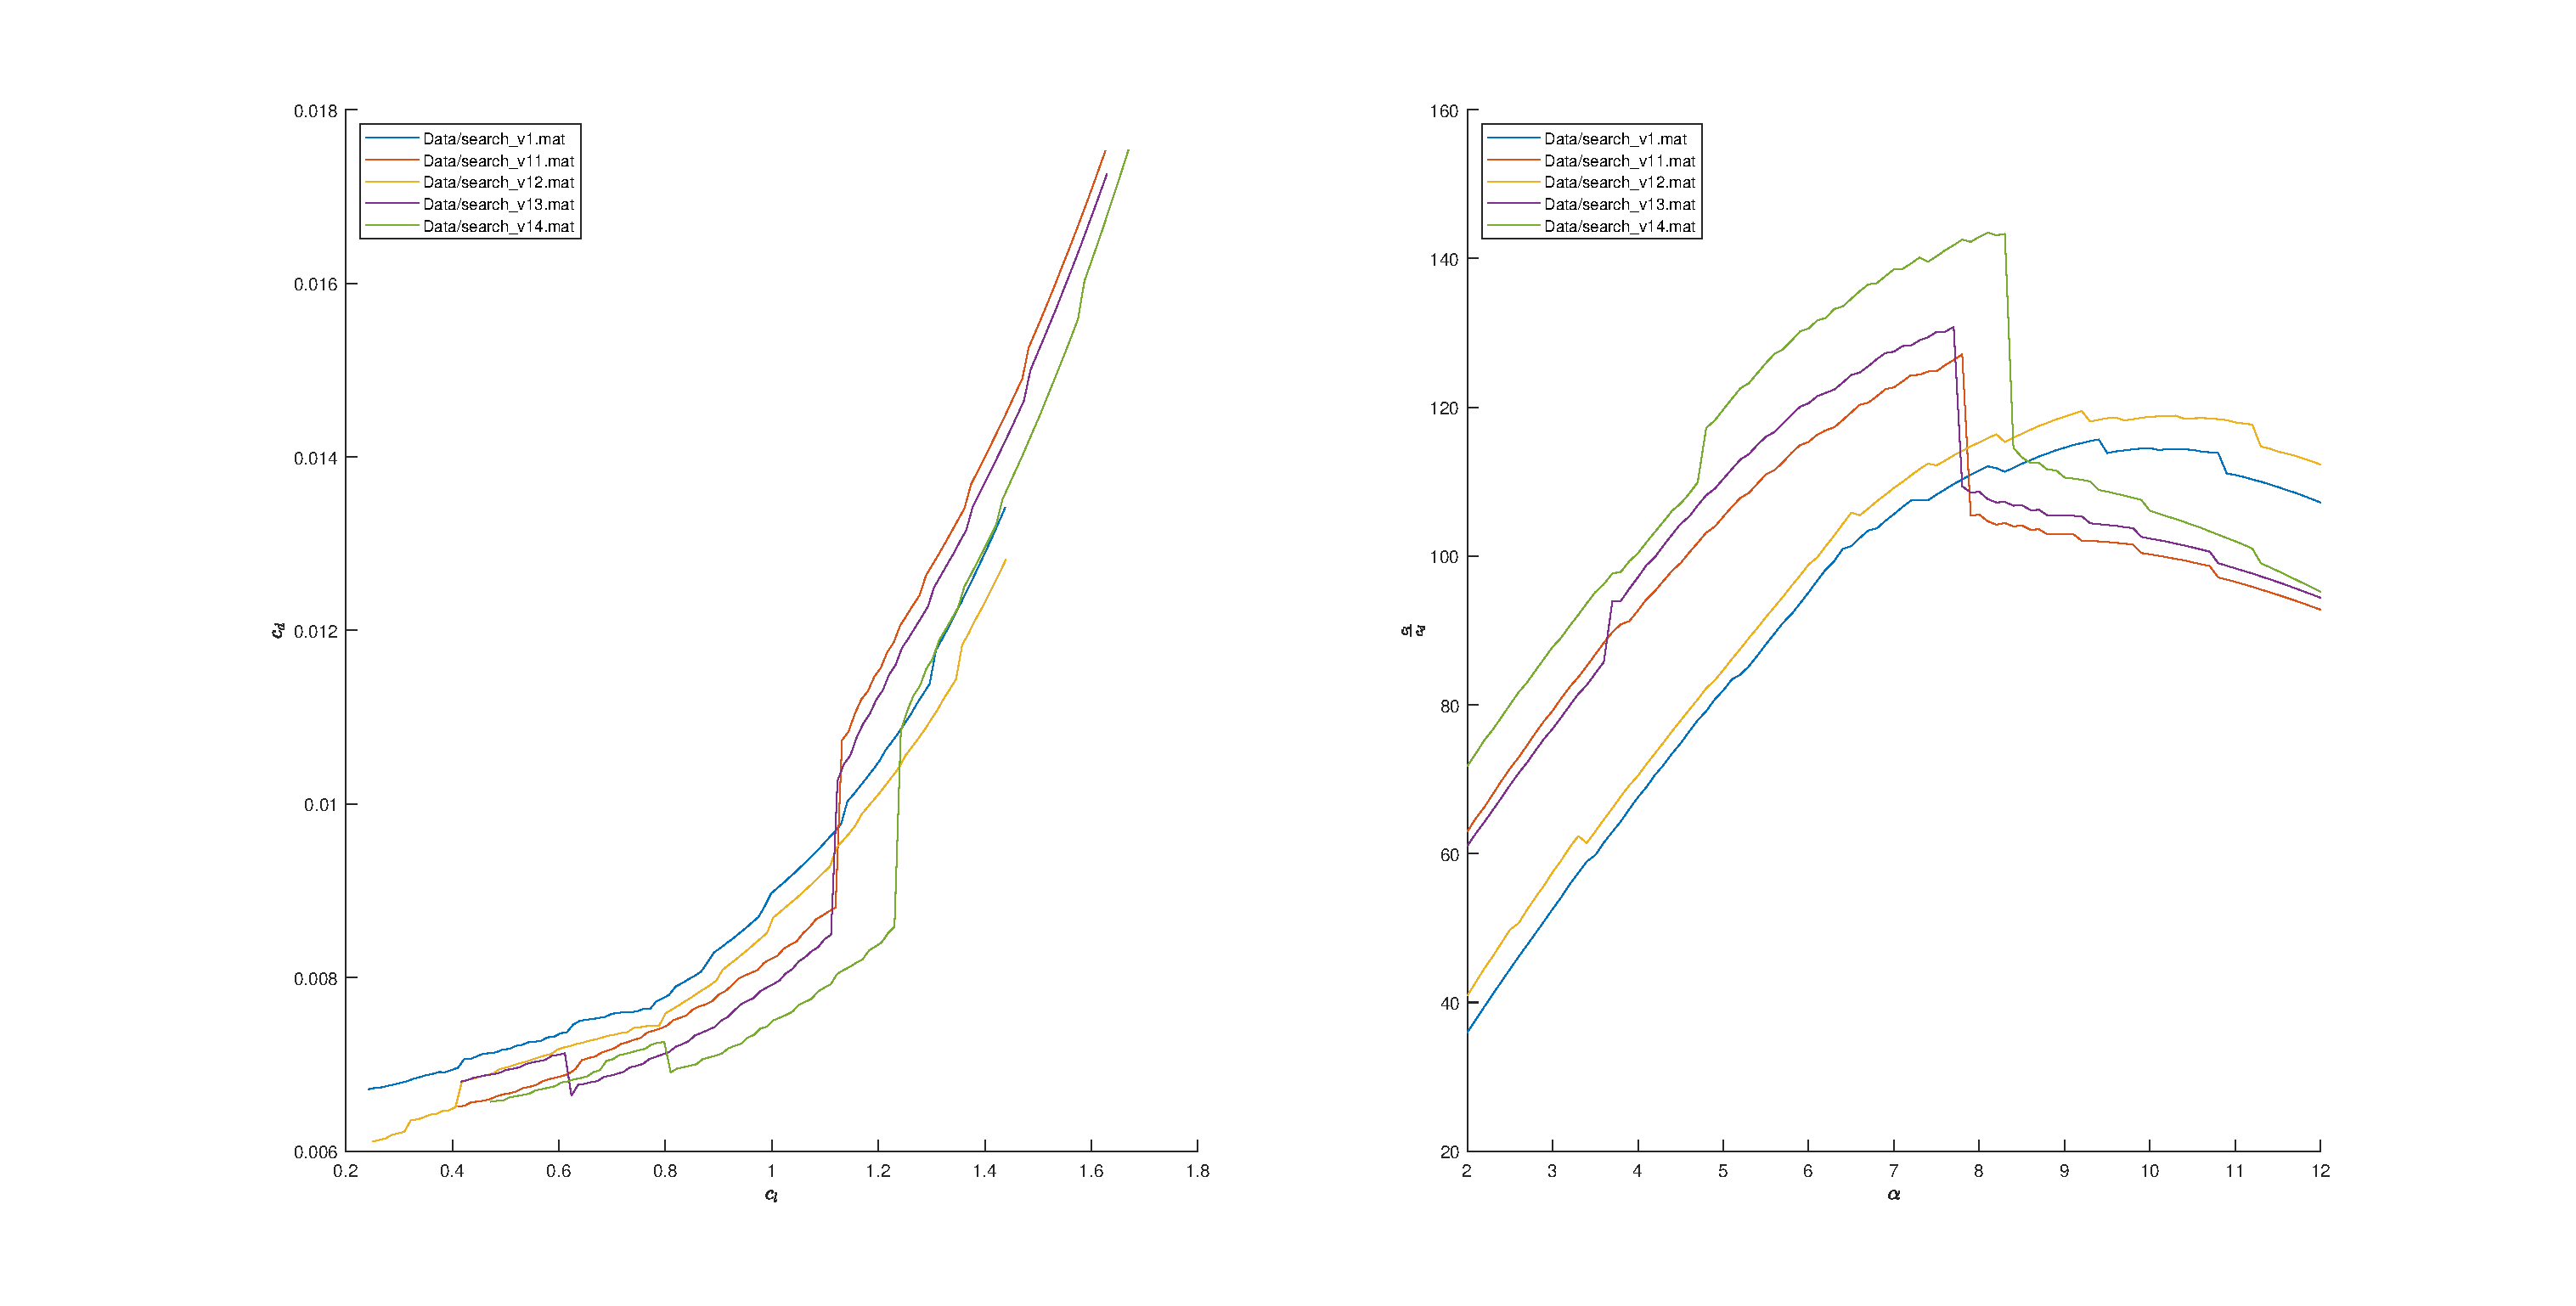
\includegraphics[width=1.2\textwidth, center]{figures/hiRe_lod_14.eps}
        \caption{Drag polar and lift to drag ratio against angle of attack}
        \label{fig:v14_lod}
    \end{subfigure}
    \caption{}
\end{figure}

\begin{figure}[H]
    \begin{subfigure}{0.49\textwidth}
        \centering
        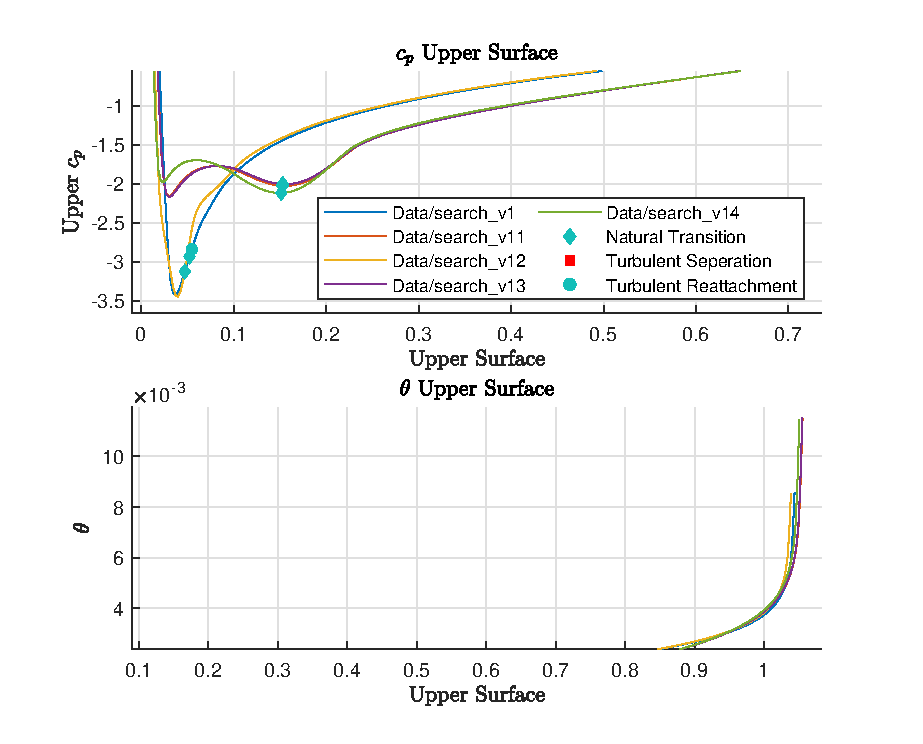
\includegraphics[width=1.1\textwidth, center]{figures/hiRe_upperprofile_14_a7.eps}
        \label{fig:v14_uprofile}
    \end{subfigure}
    \begin{subfigure}{0.49\textwidth}
        \centering
        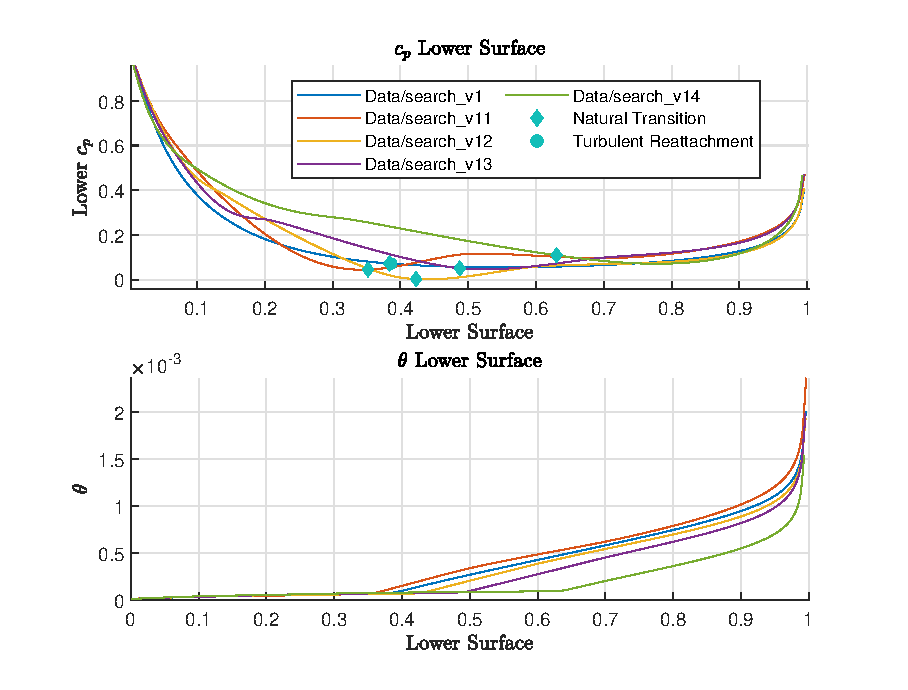
\includegraphics[width=1.1\textwidth, center]{figures/hiRe_lowerprofile_14_a7.eps}
        \label{fig:v14_lprofile}
    \end{subfigure}
    \caption{Upper and lower surface pressure coefficient and momentum thickness profiles for $\alpha = 7^\circ$}
\end{figure}

\begin{figure}[H]
    \centering
    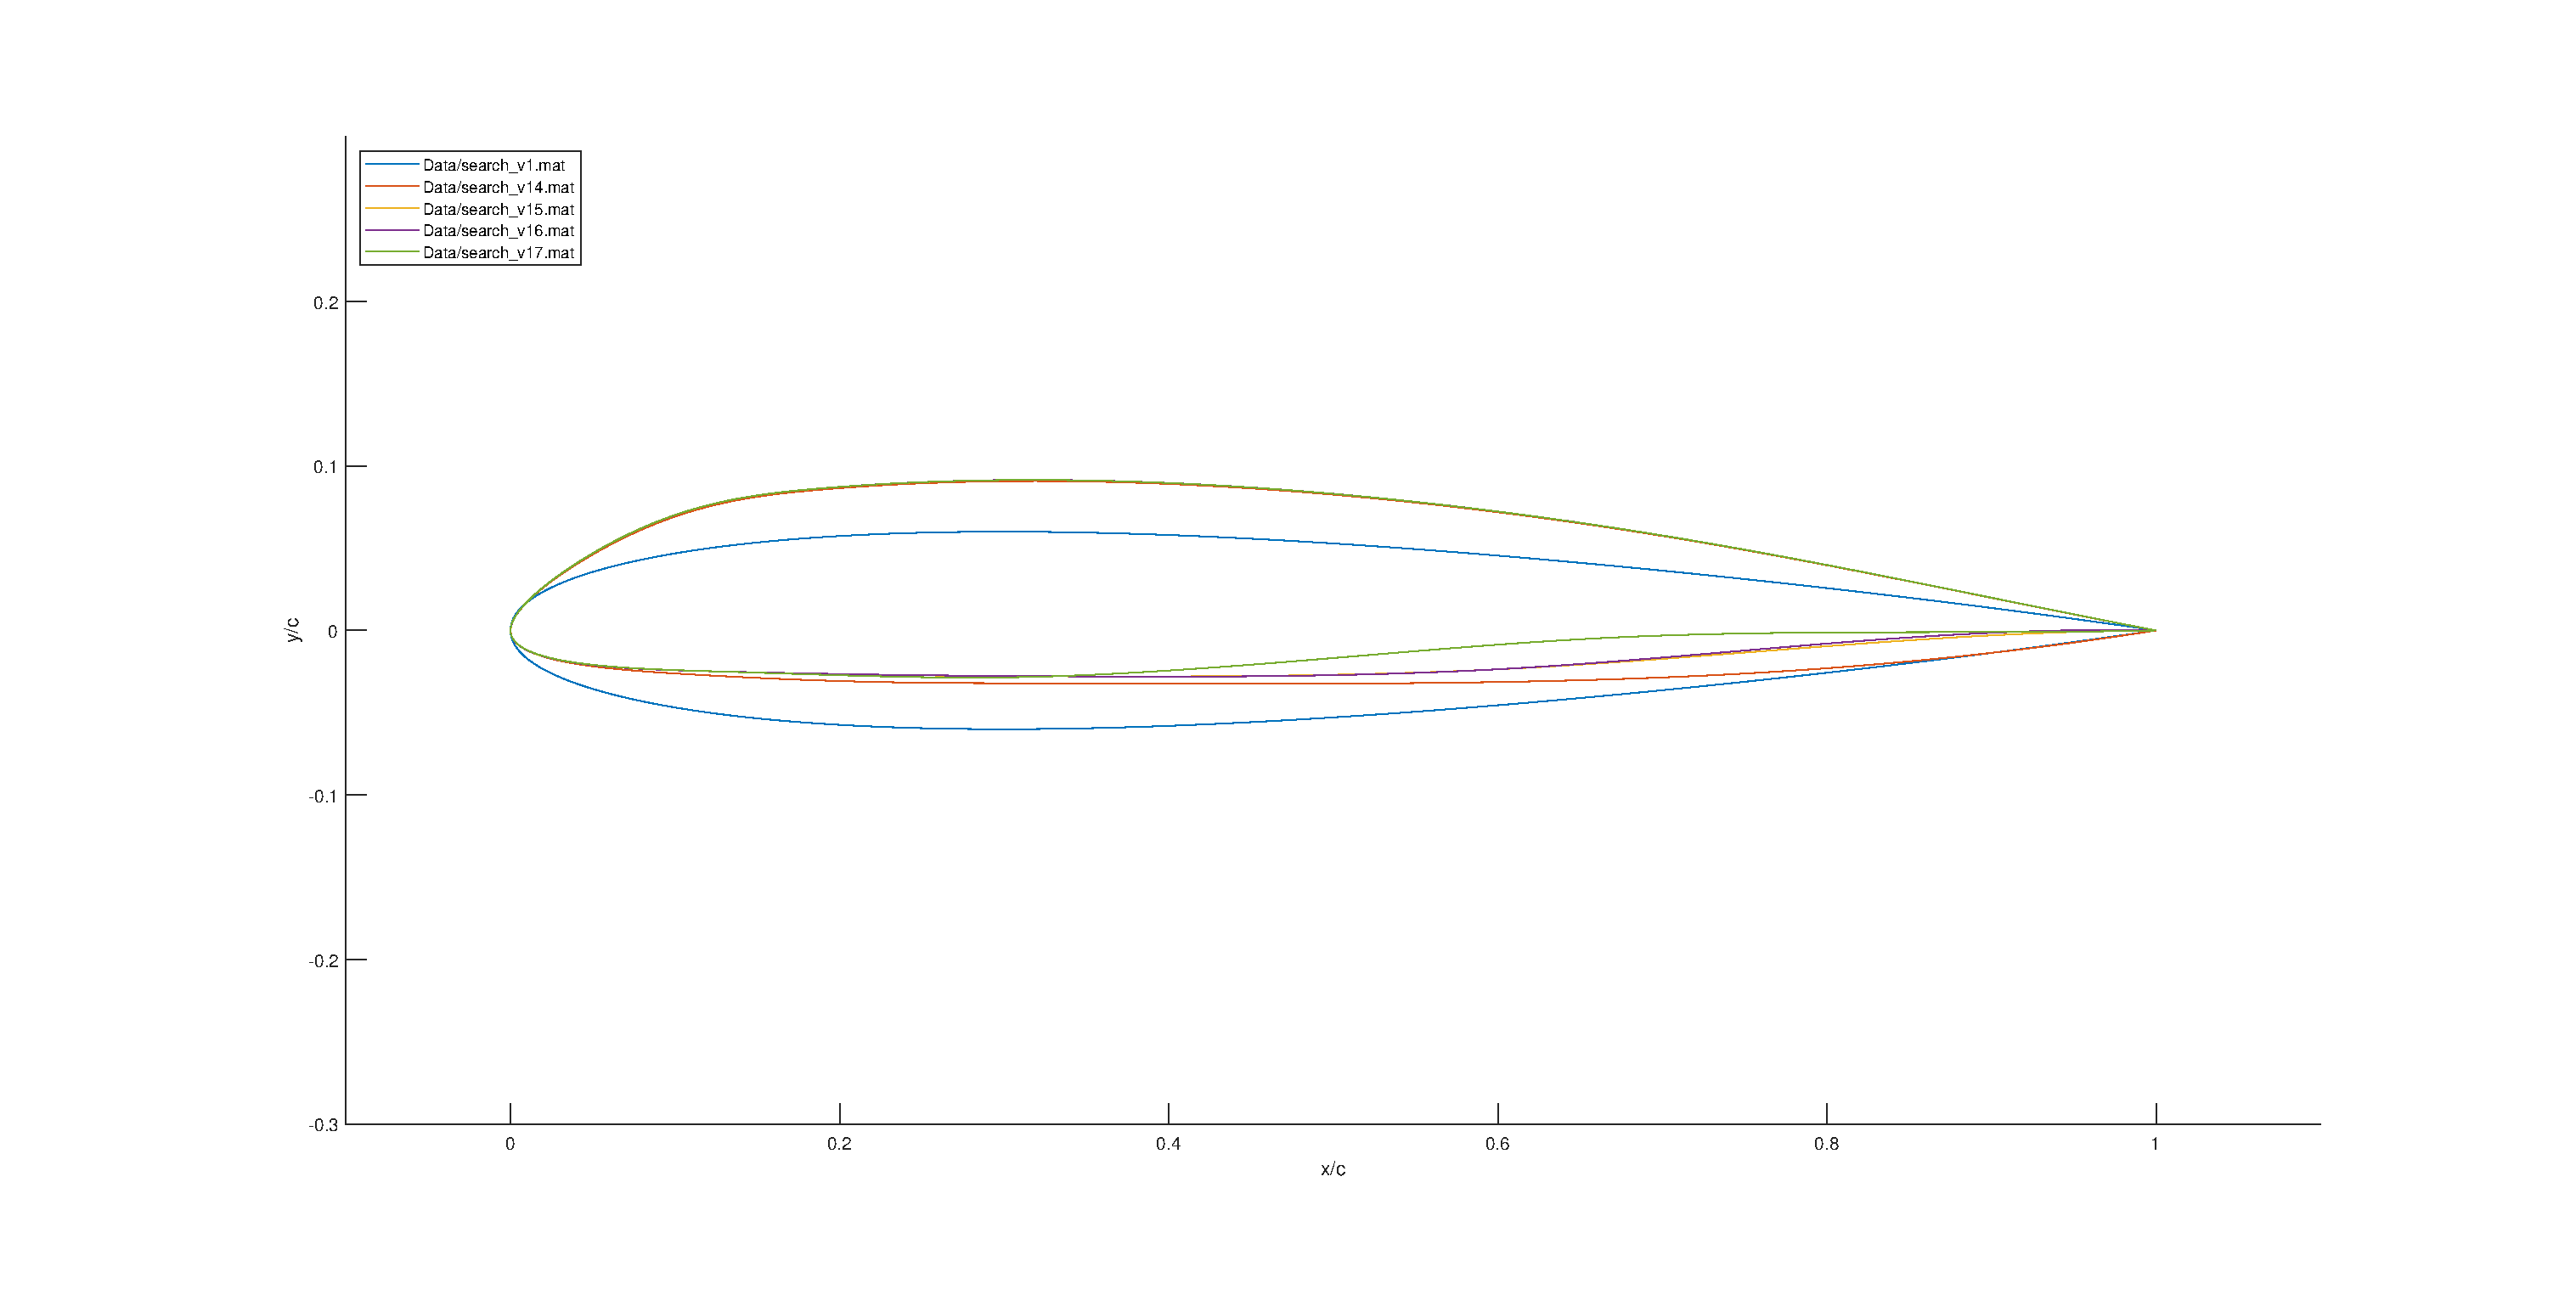
\includegraphics[width=0.8\textwidth]{figures/hiRe_geometry_17.eps}
    \caption{Airfoil}
    \label{fig:v17_geometry}
\end{figure}

\begin{figure}[H]
    \centering
    \begin{subfigure}{0.45\textwidth}
        \centering
        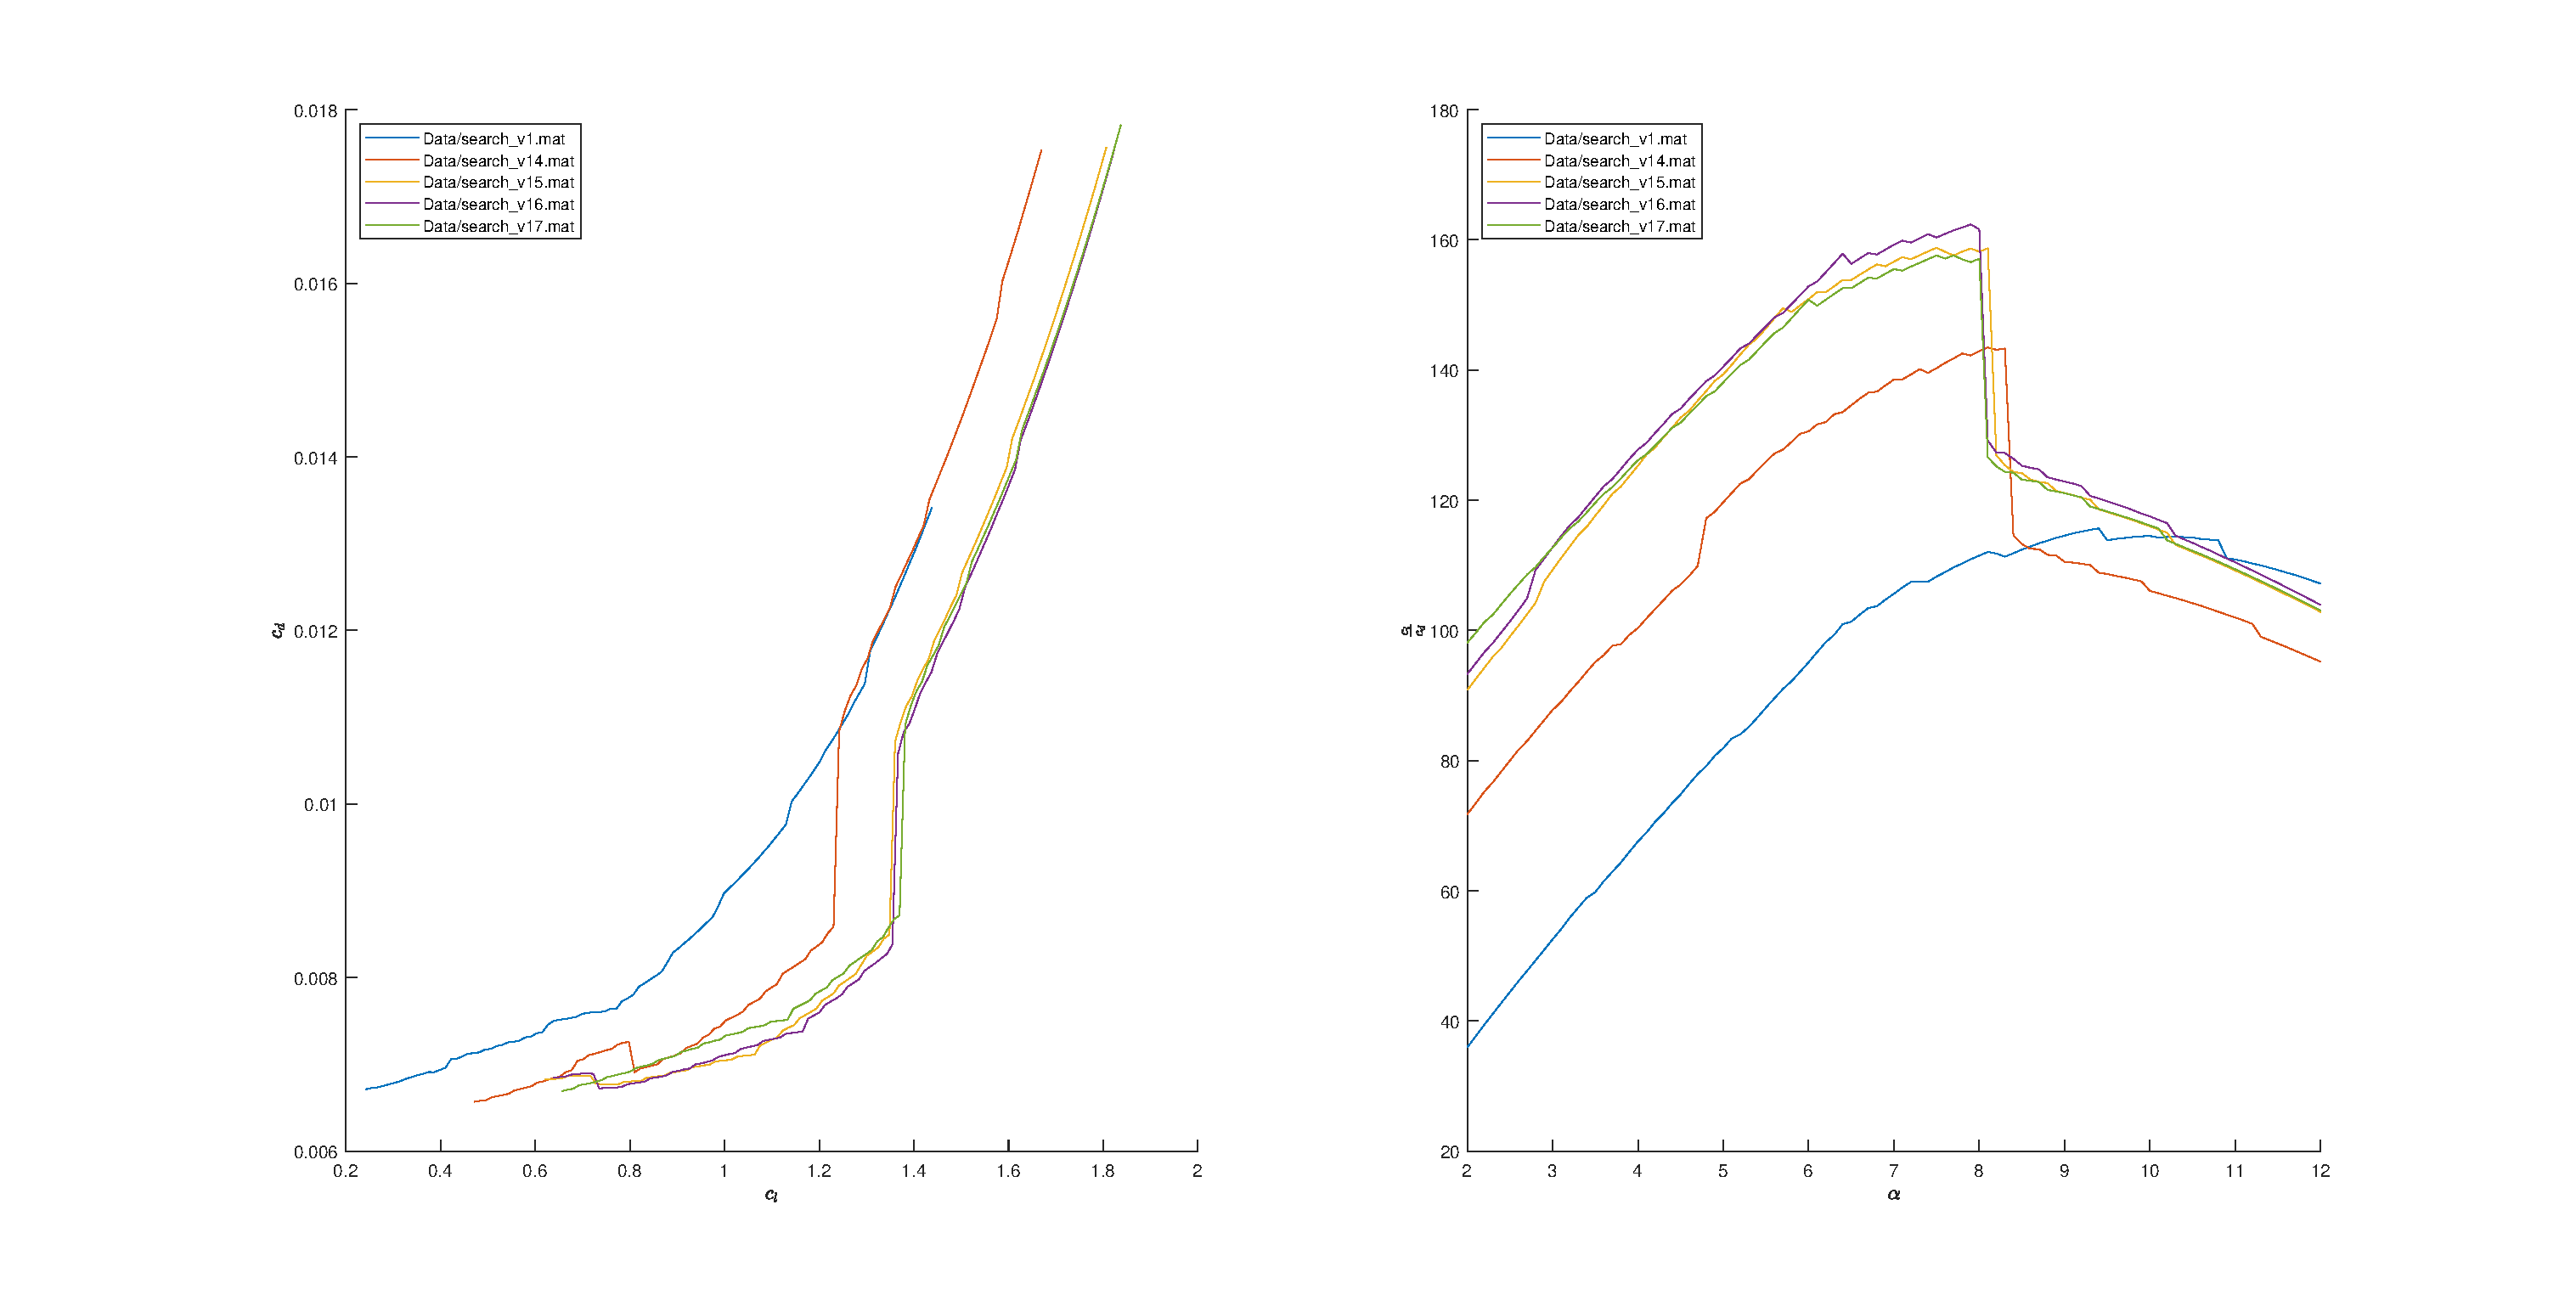
\includegraphics[width=1.2\textwidth, center]{figures/hiRe_lod_17.eps}
        \caption{Airfoil}
        \label{fig:v17_lod}
    \end{subfigure}
    \begin{subfigure}{0.54\textwidth}
        \centering
        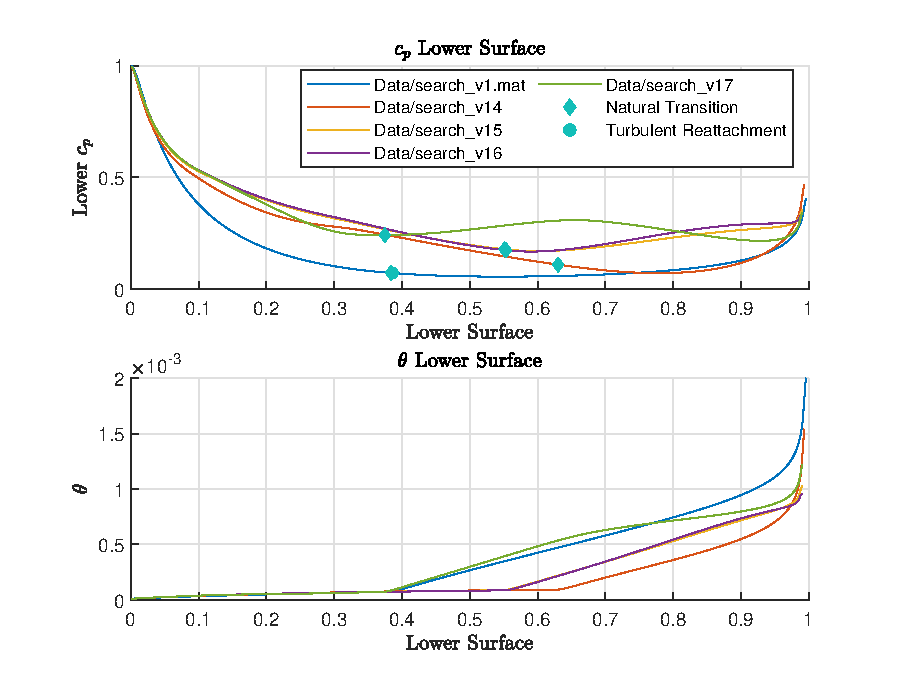
\includegraphics[width=0.99\textwidth]{figures/hiRe_lowerprofile_17_a7.eps}
        \caption{Pressure coefficient and momentum thickness profiles for $\alpha = 7^\circ$}
        \label{fig:v17_lprofile}
    \end{subfigure}
    \caption{Performance of design iterations 14-17 and their upper surface boundary layer profiles}
\end{figure}

\begin{figure}[H]
    \centering
    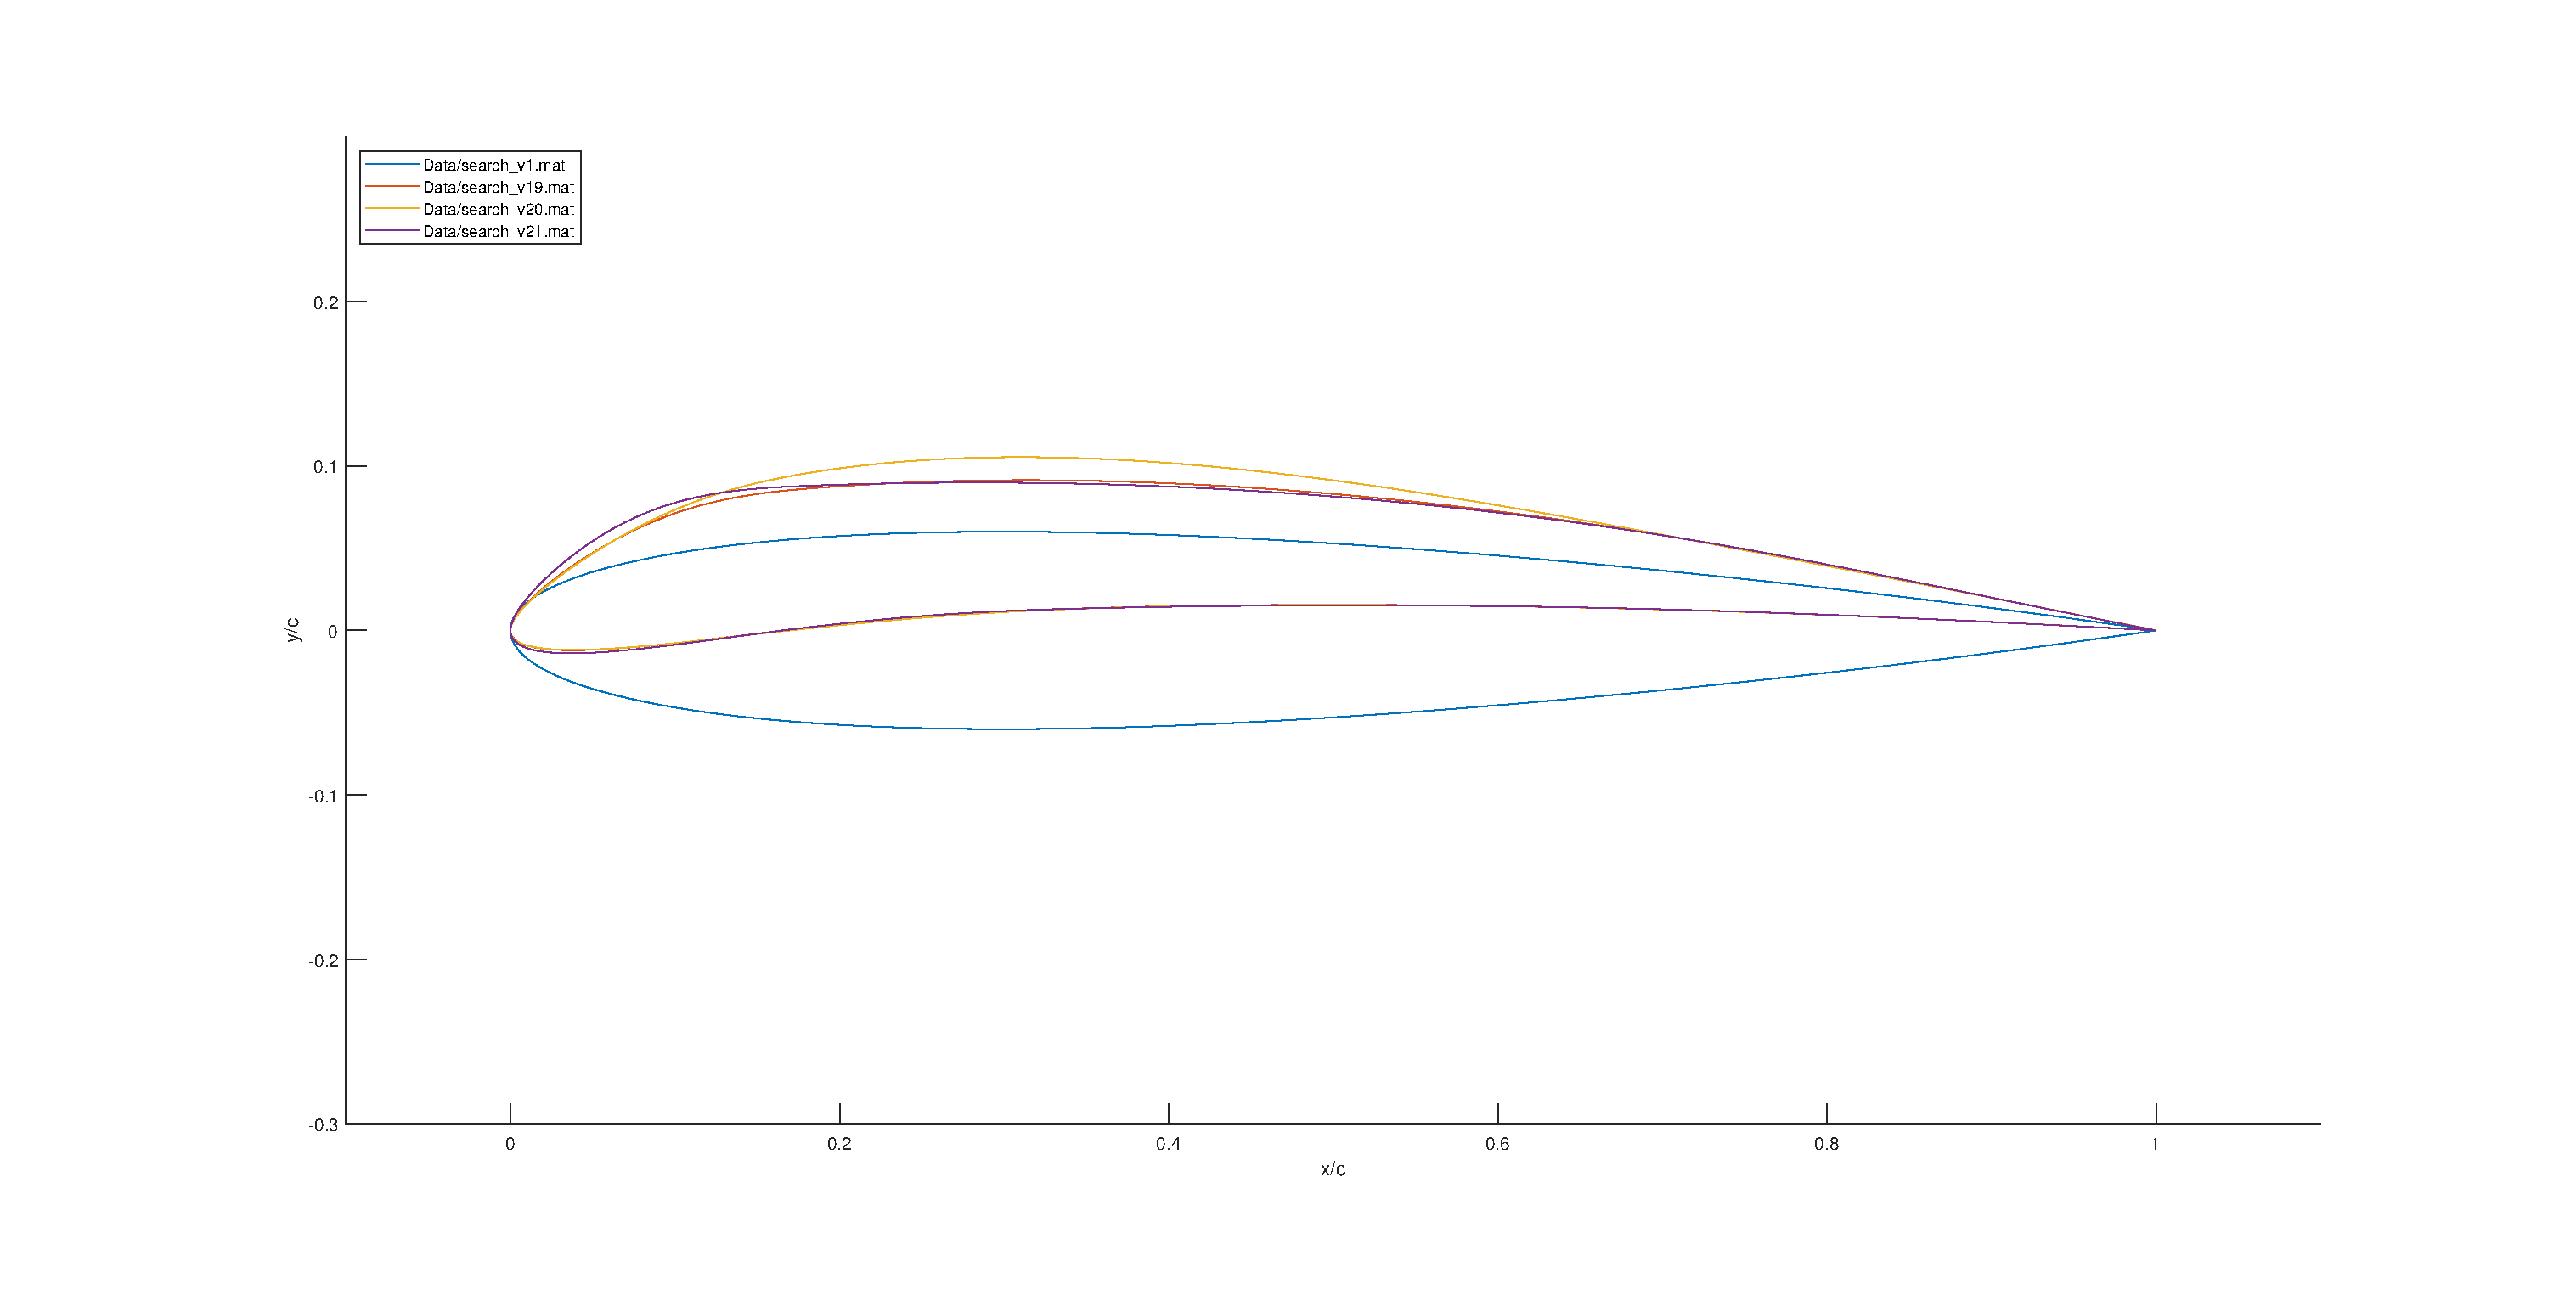
\includegraphics[width=0.8\textwidth]{figures/hiRe_geometry_21.eps}
    \caption{Airfoil}
    \label{fig:v21_geometry}
\end{figure}

\begin{figure}[H]
    \centering
    \begin{subfigure}{0.45\textwidth}
        \centering
        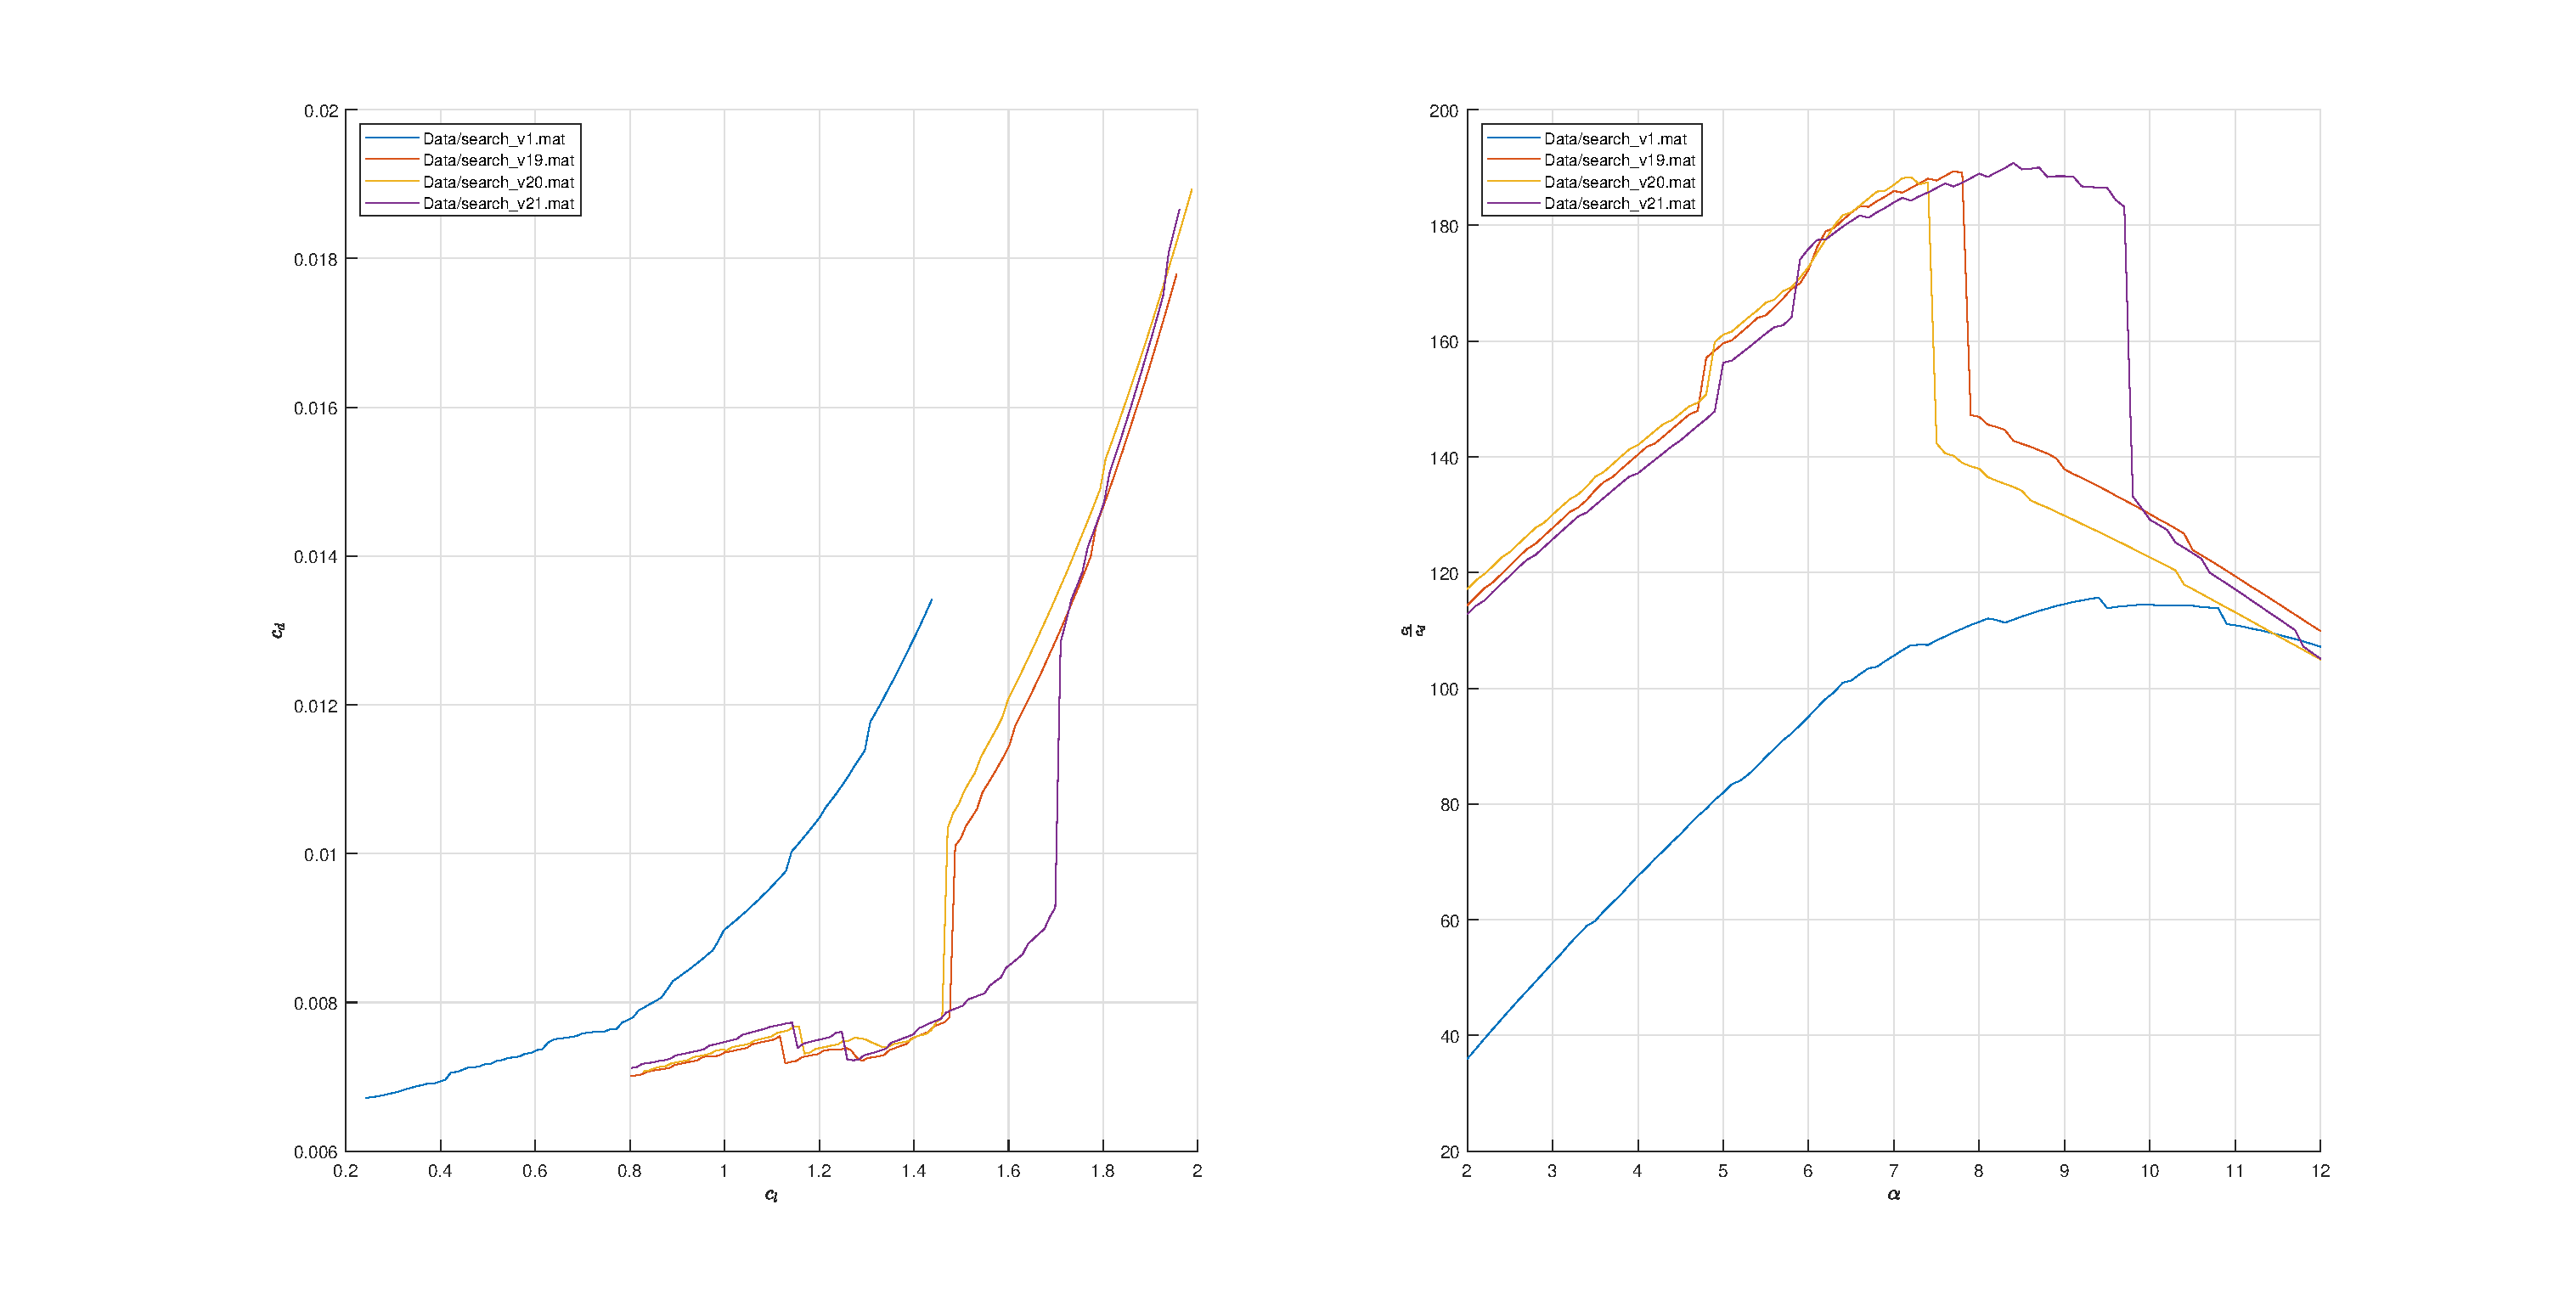
\includegraphics[width=1.2\textwidth, center]{figures/hiRe_lod_21.eps}
        \caption{Airfoil}
        \label{fig:v21_lod}
    \end{subfigure}
    \begin{subfigure}{0.54\textwidth}
        \centering
        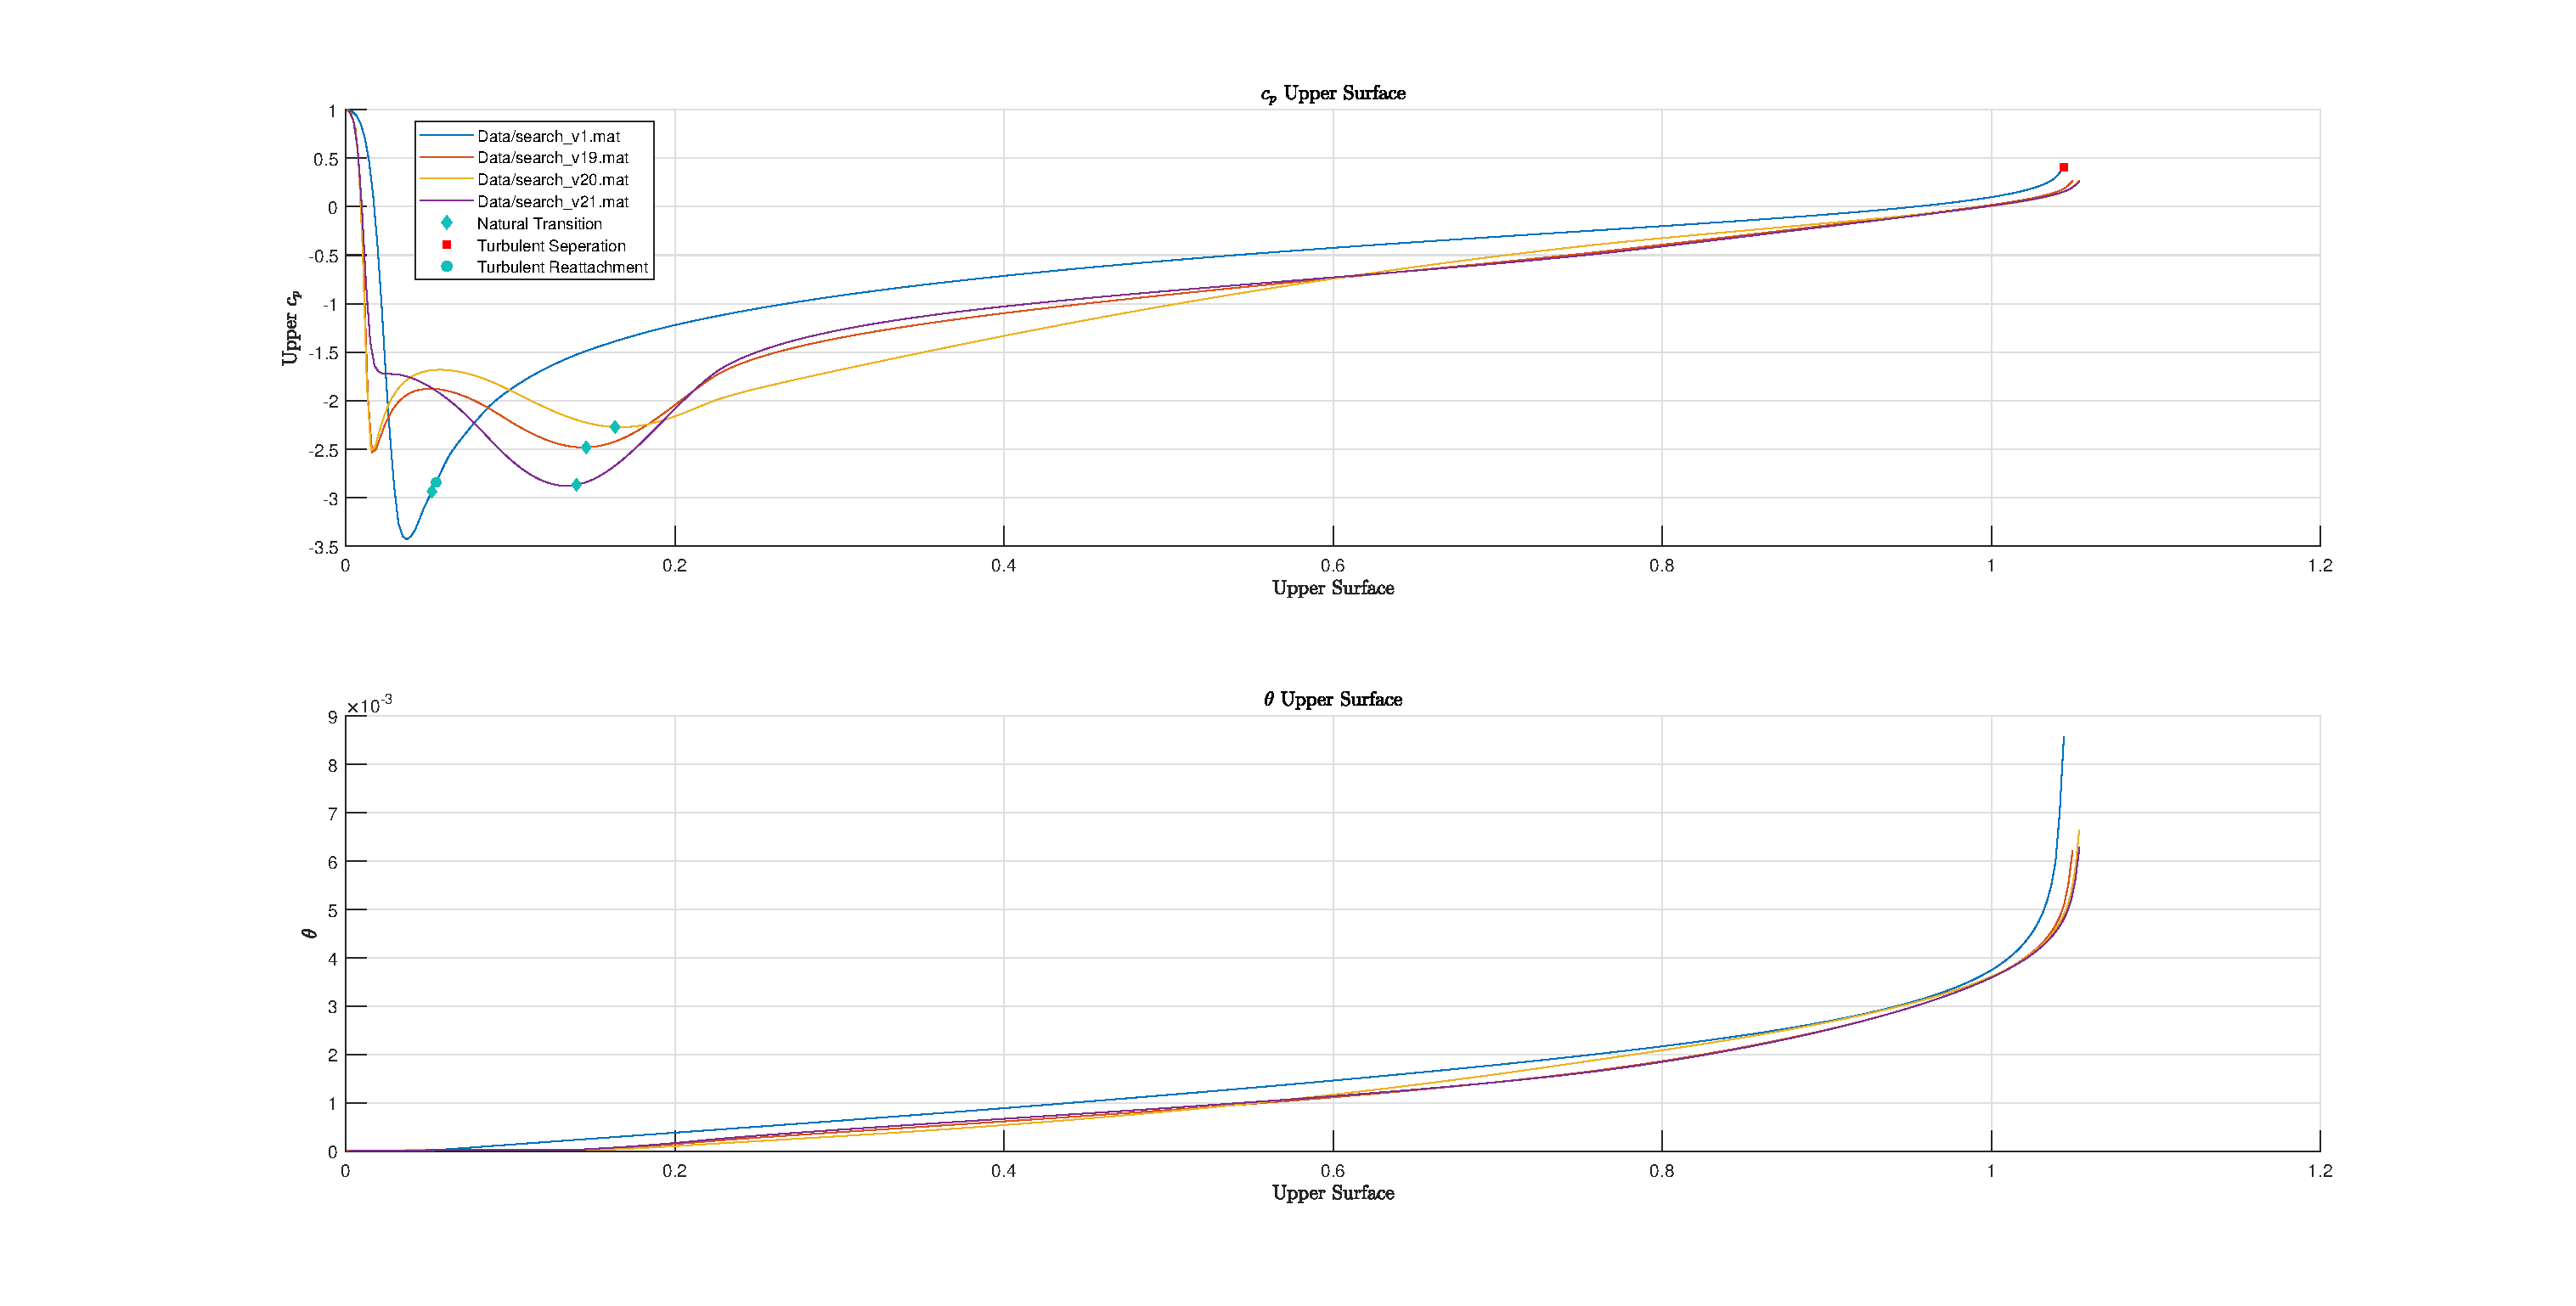
\includegraphics[width=0.6\textwidth]{figures/hiRe_upperprofile_21_a7.eps}
        \caption{Pressure coefficient and momentum thickness profiles for $\alpha = 7^\circ$}
        \label{fig:v21_uprofile}
    \end{subfigure}
    \caption{Performance of design iterations 14-17 and their upper surface boundary layer profiles}
\end{figure}

\subsection{Low Reynolds Number}


\end{document}